\documentclass{article}

\usepackage{amsmath}
\usepackage{amsfonts}
\usepackage{amssymb}
\usepackage{graphicx}
\usepackage{float}
\usepackage{geometry}

\geometry{
  top=2cm,    % top margin
  bottom=2cm, % bottom margin
  left=2cm, % left margin
  right=2cm % right margin
}

\usepackage[polish]{babel}
\usepackage[utf8]{inputenc}
\usepackage{polski}
\usepackage[T1]{fontenc}

\usepackage{url}

\usepackage{minted}

\newenvironment{fact}[1]{%
    \trivlist
    \item[\hskip\labelsep\textbf{Fakt. #1.}]
    \ignorespaces
}{%
    \endtrivlist
}

\title{Metody Probabilistyczne i Statystyka}
\author{Zadanie domowe 2}
\date{Rafał Włodarczyk 2024-11-24}

\begin{document}
\maketitle

\tableofcontents

\section{Zadanie 1}

\subsection{Technologie wykorzystane w symulacji}

Do realizacji zadania wykorzystałem język \textit{rust}. Liczby pseudolosowe są generowane za pomocą biblioteki \textit{rand\_mt} (Mersenne Twister). Wykresy stworzyłem za pomocą narzędzia \textit{matplotlib}. 

\subsubsection{Pojedyncza symulacja}

Do uzyskania wyników wszystkich pomiarów, każdorazowo losowany jest urna do której zostanie wrzucona kula. W trakci symulacji mierzone są ilości urn z $0$, $1$ oraz $2$ kulami, oraz $u(n)$ w tysięcznej iteracji. Po jej zakończeniu, czyli po tym, gdy w każdej z urn znajdują się co najmniej dwie kule zliczana jest różnica $d(n)-c(n)$.

\begin{minted}[fontsize=\small, linenos]{rust}
let mut bins = simulation::create_bins(n);
let mut metrics = types::Metrics::new();
let mut count_0: u32 = n; // count occurrences of 0
let mut count_1: u32 = 0; // count occurrences of 1
let mut count_2: u32 = 0; // count occurrences of 2

let mut i = 0;
while count_2 != n || count_1 != n {
let selected = simulation::randomly_place_ball(&mut bins, n);

match bins[selected] {
    1 => {
        count_1 += 1;
        count_0 -= 1;
    }
    2 => count_2 += 1,
    _ => {}
}

// [...] all checks

}
\end{minted}

\subsubsection{Grupa symulacji}

Dla każdego $n\in\{1000,2000,...,100000\}$ wykonuje $k=50$ niezależnych powtórzeń a następnie uśredniam wyniki każdej zbieranej wartości. W celu usprawnienia prędkości jej wykonywania użyłem biblioteki \textit{rayon}, która pozwoliła mi wykonywać symulację na wielu rdzeniach CPU.

\begin{minted}[fontsize=\small, linenos]{rust}
const SAME_SIM_REPS: usize = 50;

// [...]

let metrics_group: Vec<types::Metrics> = (0..SAME_SIM_REPS)
.into_par_iter()
.map(|_k| {
    // [...] single simulation
})
.collect();
\end{minted}

\subsection{Wykresy}

\subsubsection{Paradoks urodzinowy - $B_n$, $\frac{b(n)}{n}$, $\frac{b(n)}{\sqrt{n}}$}

\begin{figure}[H]
    \centering
    \begin{minipage}{0.24\textwidth}
        \centering
        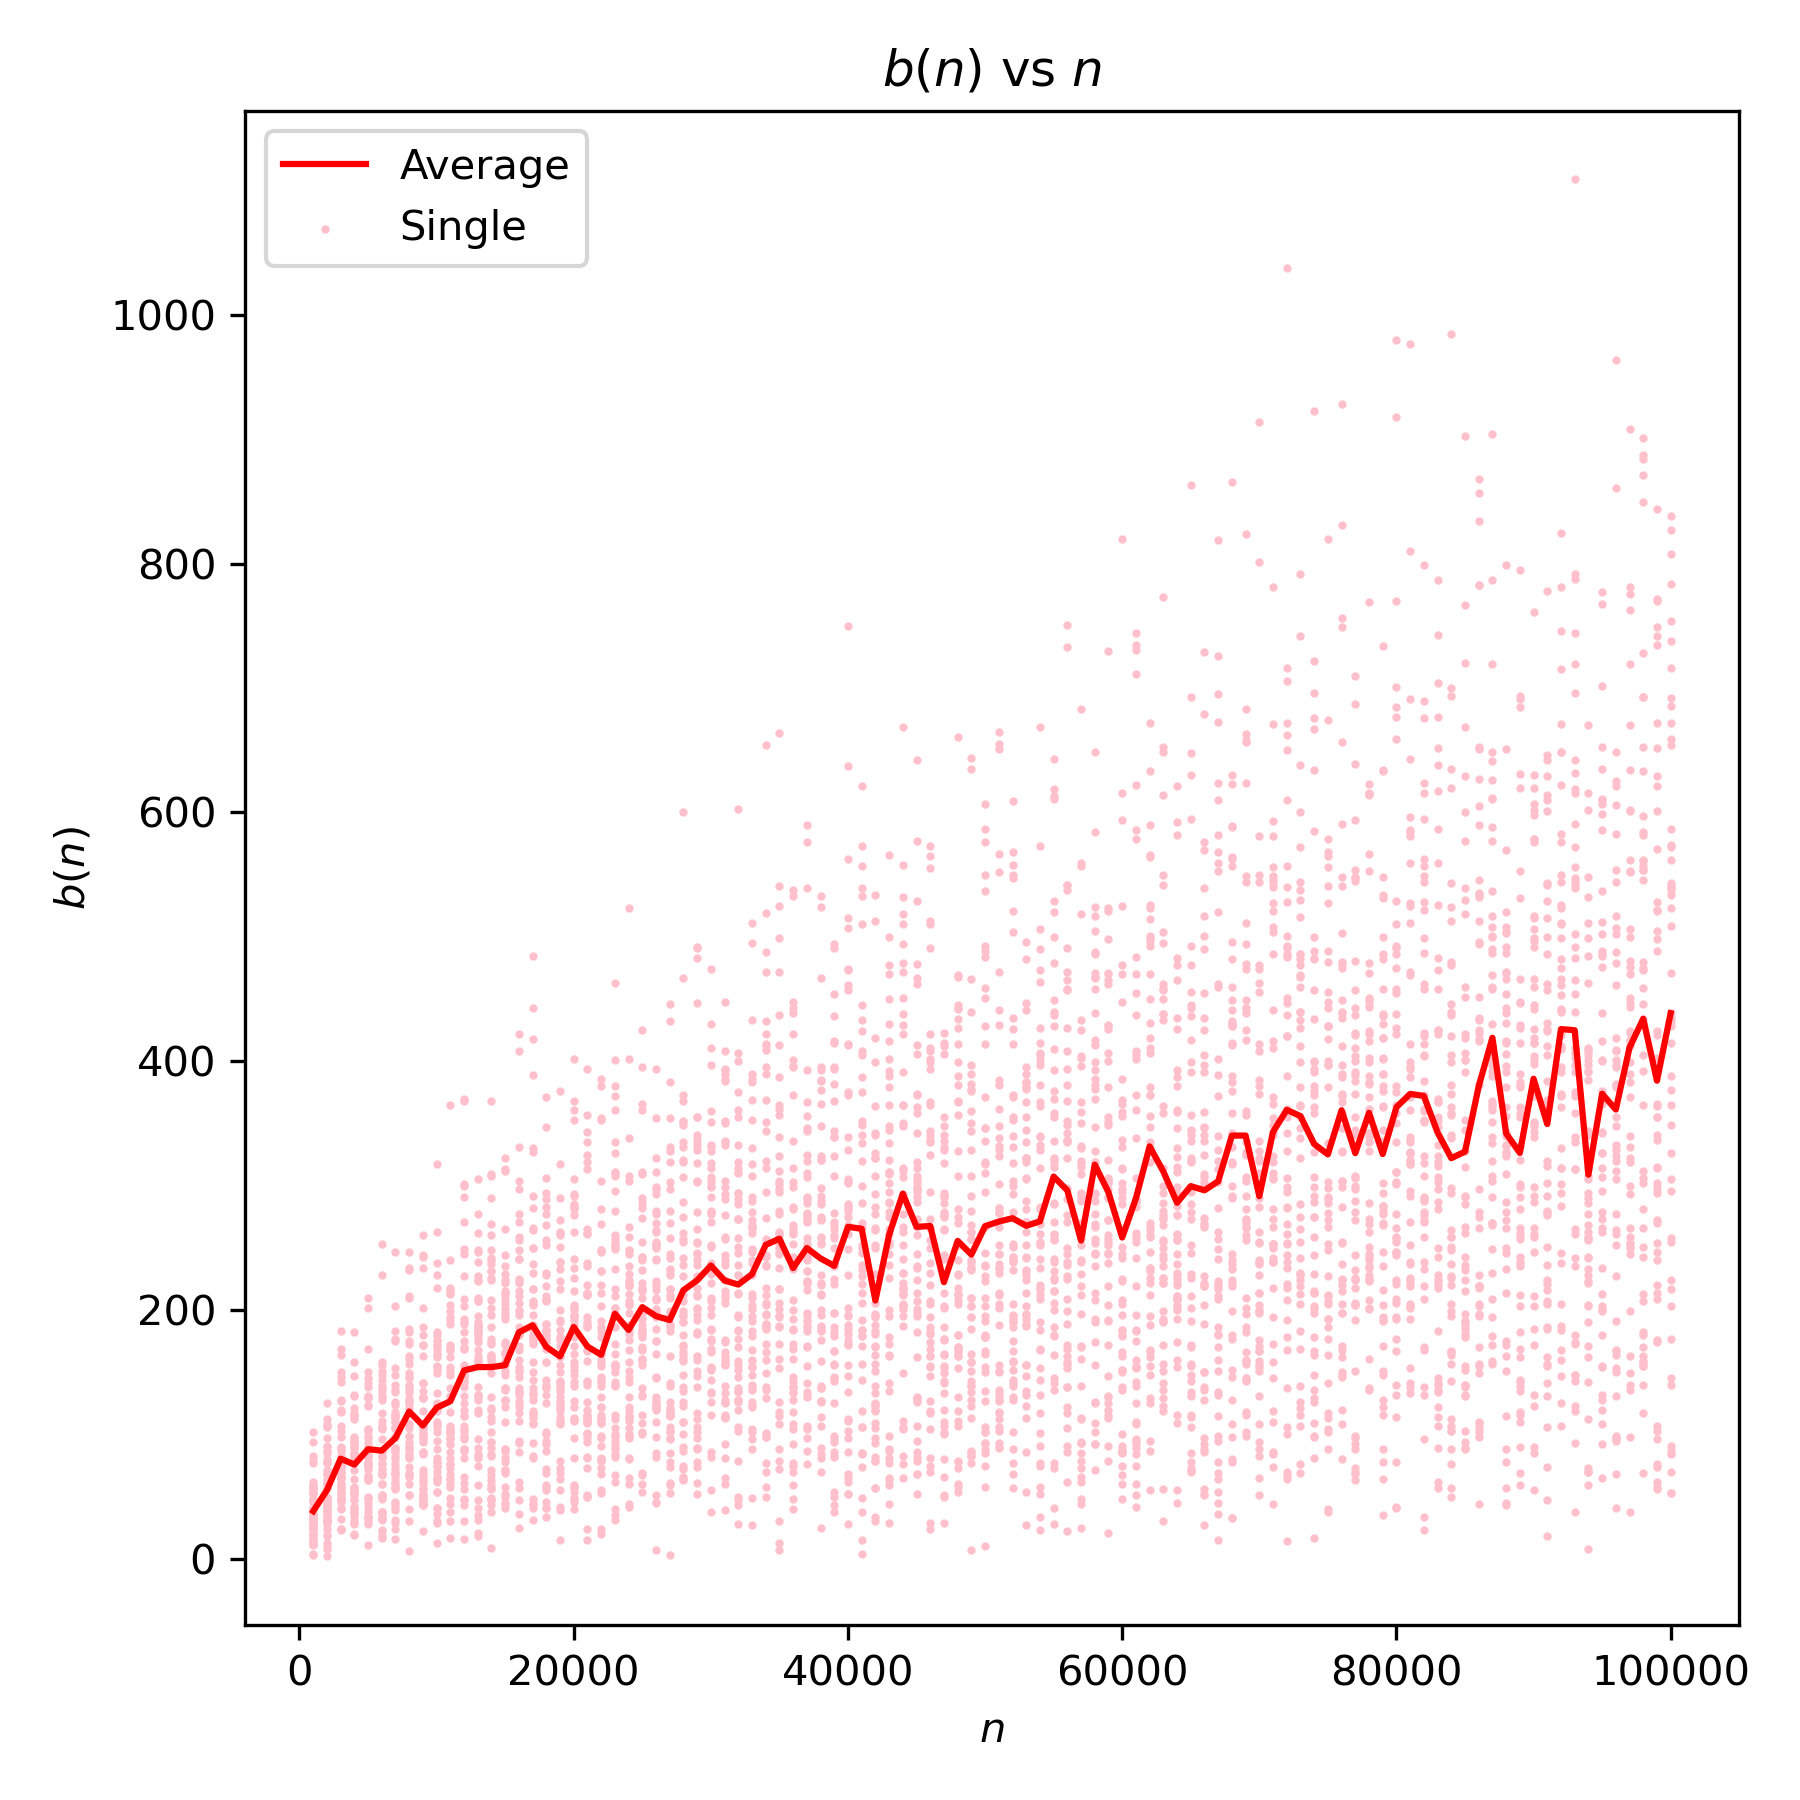
\includegraphics[width=\linewidth]{b_factor_vs_n.png}
        \caption{$B(n)$}
    \end{minipage}
    \begin{minipage}{0.24\textwidth}
        \centering
        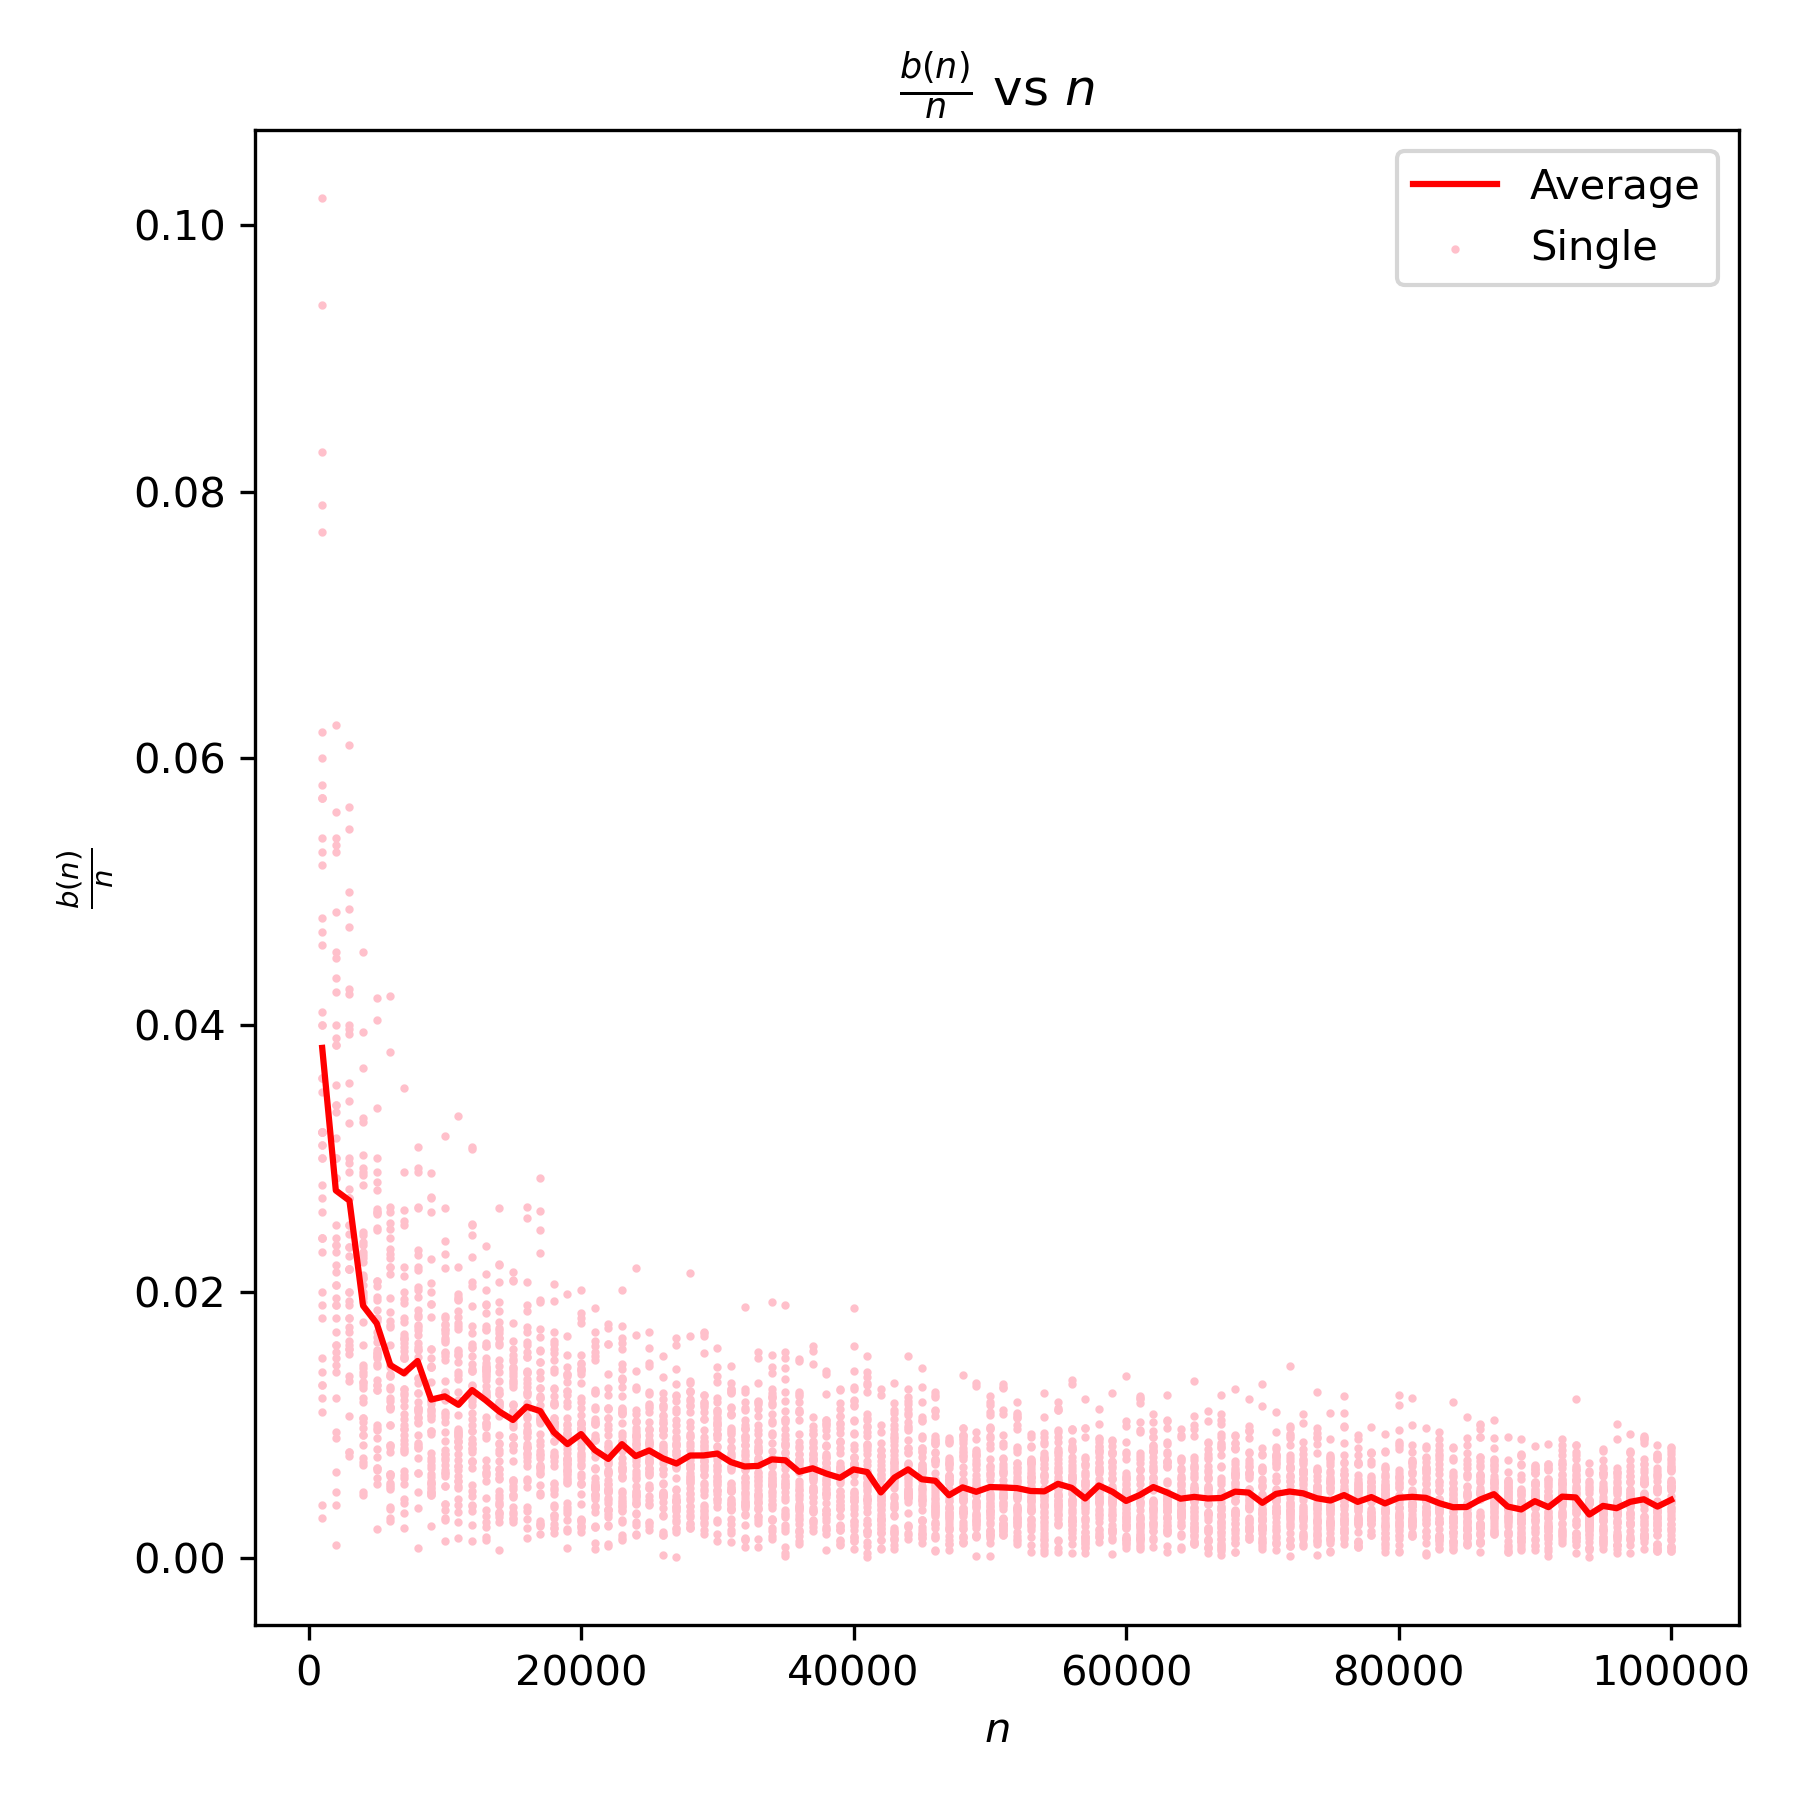
\includegraphics[width=\linewidth]{b_factor_over_n_vs_n.png}
        \caption{$\frac{b(n)}{n}$}
    \end{minipage}
    \begin{minipage}{0.24\textwidth}
        \centering
        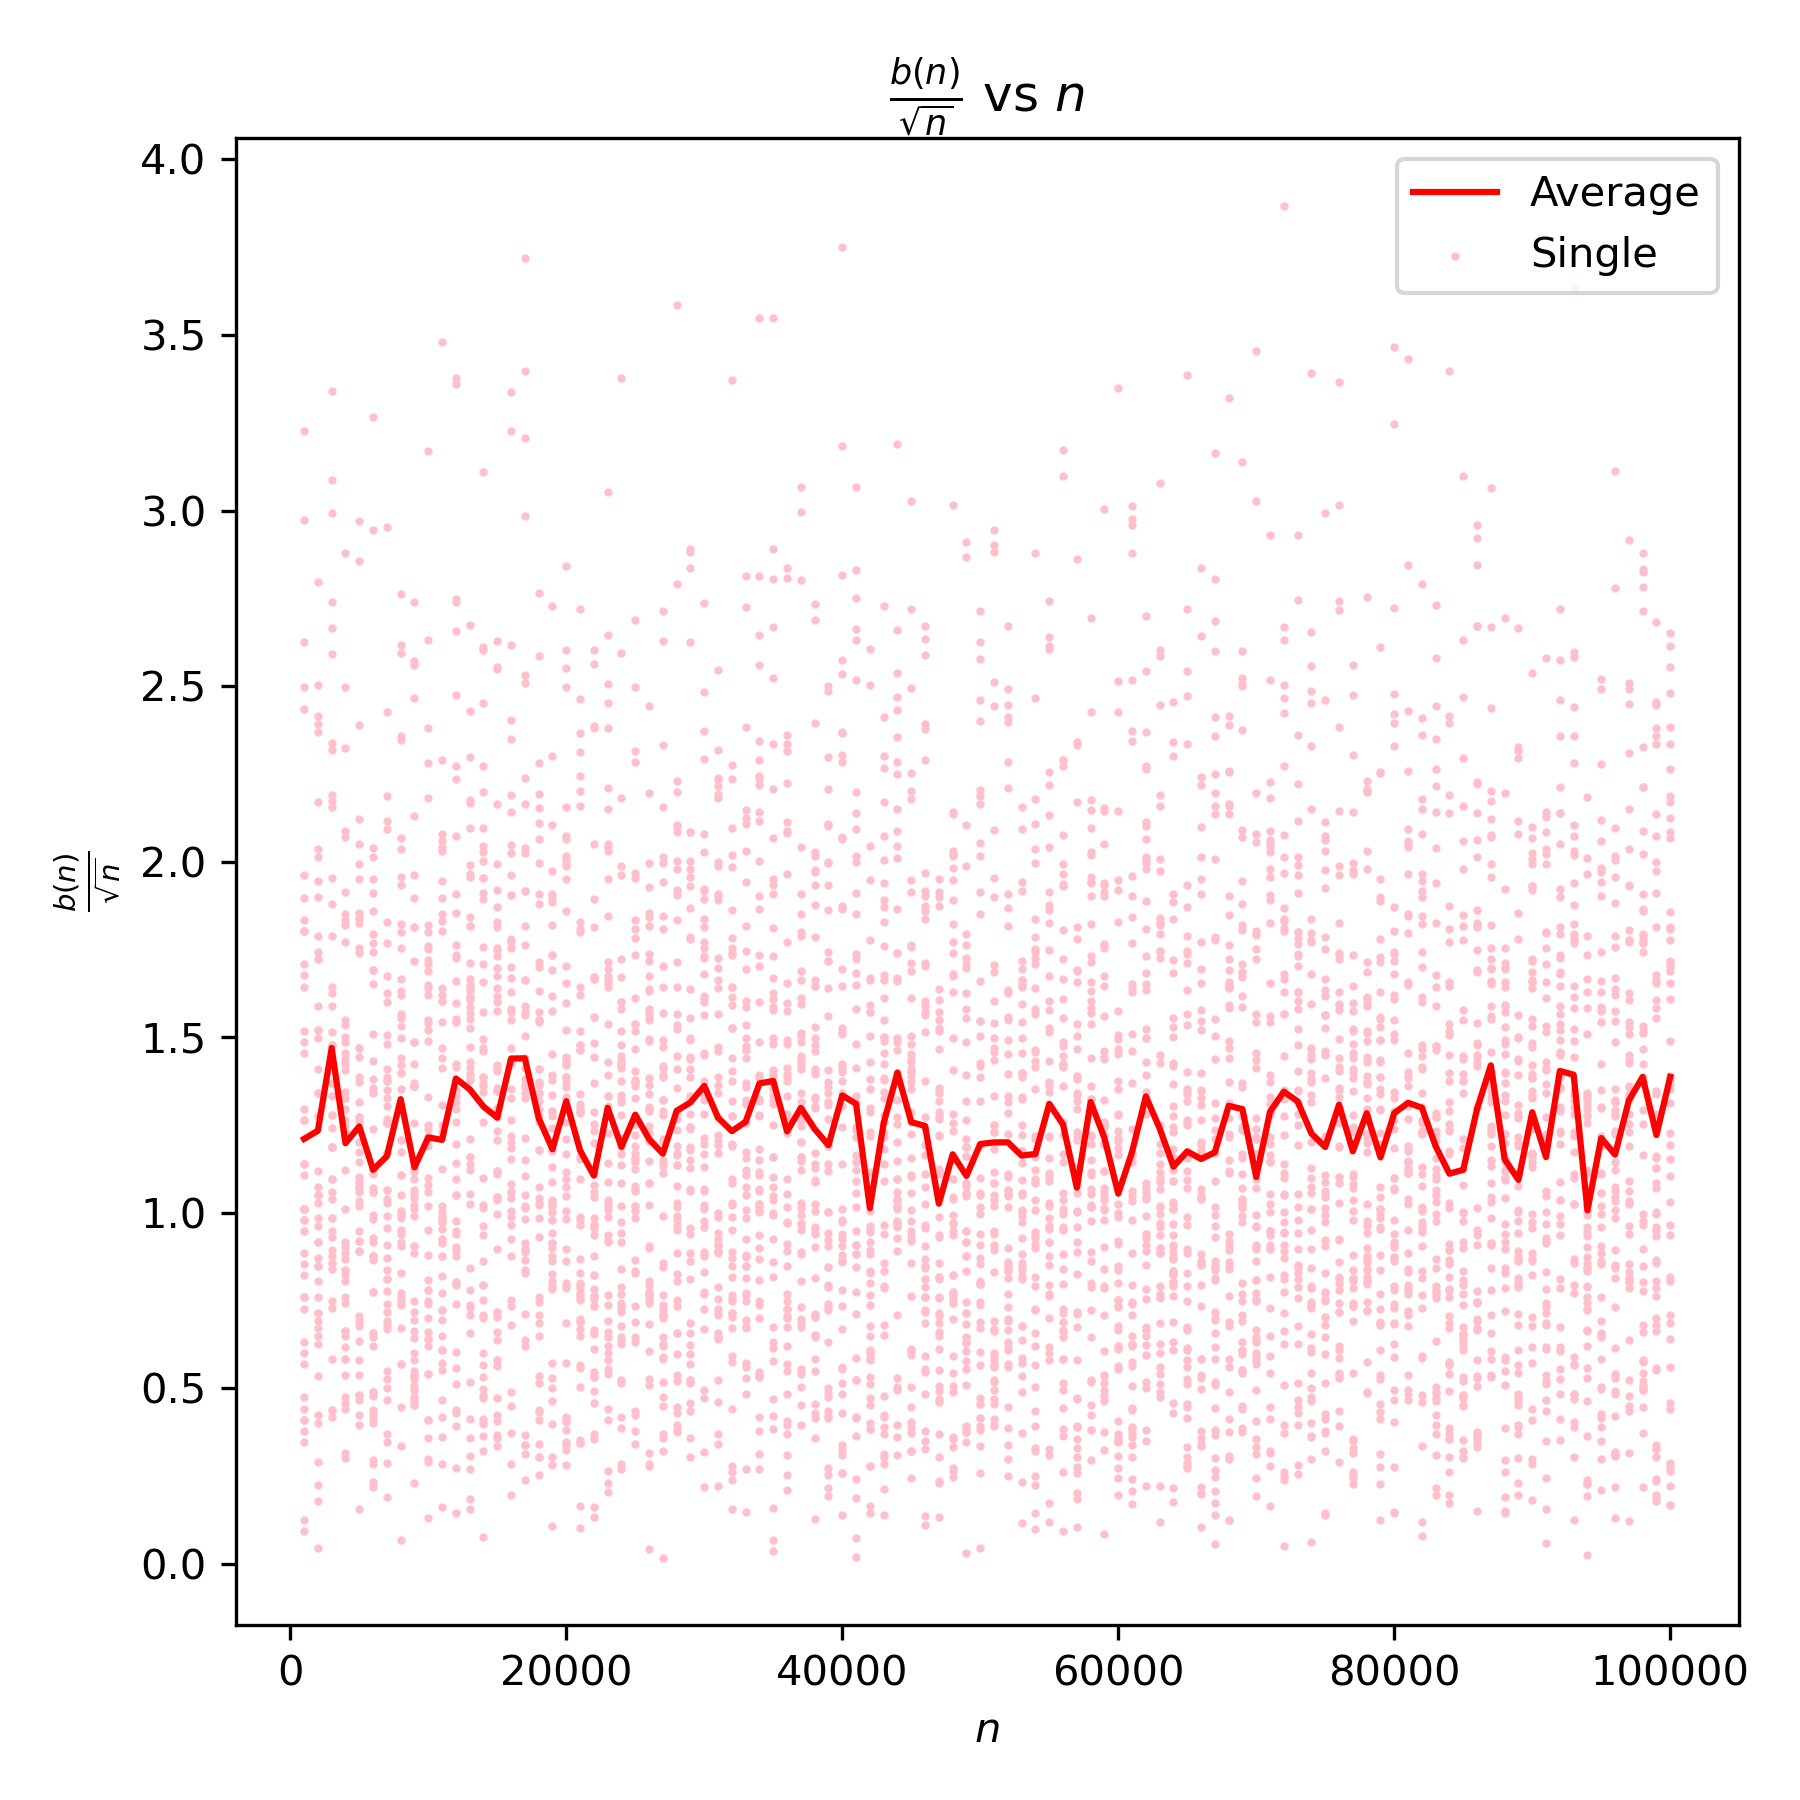
\includegraphics[width=\linewidth]{b_factor_over_sqrt_n_vs_n.png}
        \caption{$\frac{b(n)}{\sqrt{n}}$}
    \end{minipage}
\end{figure}


\subsubsection{Puste urny po $n$ rzutach - $U_n, \frac{u(n)}{n}$}

\begin{figure}[H]
    \centering
    \begin{minipage}{0.24\textwidth}
        \centering
        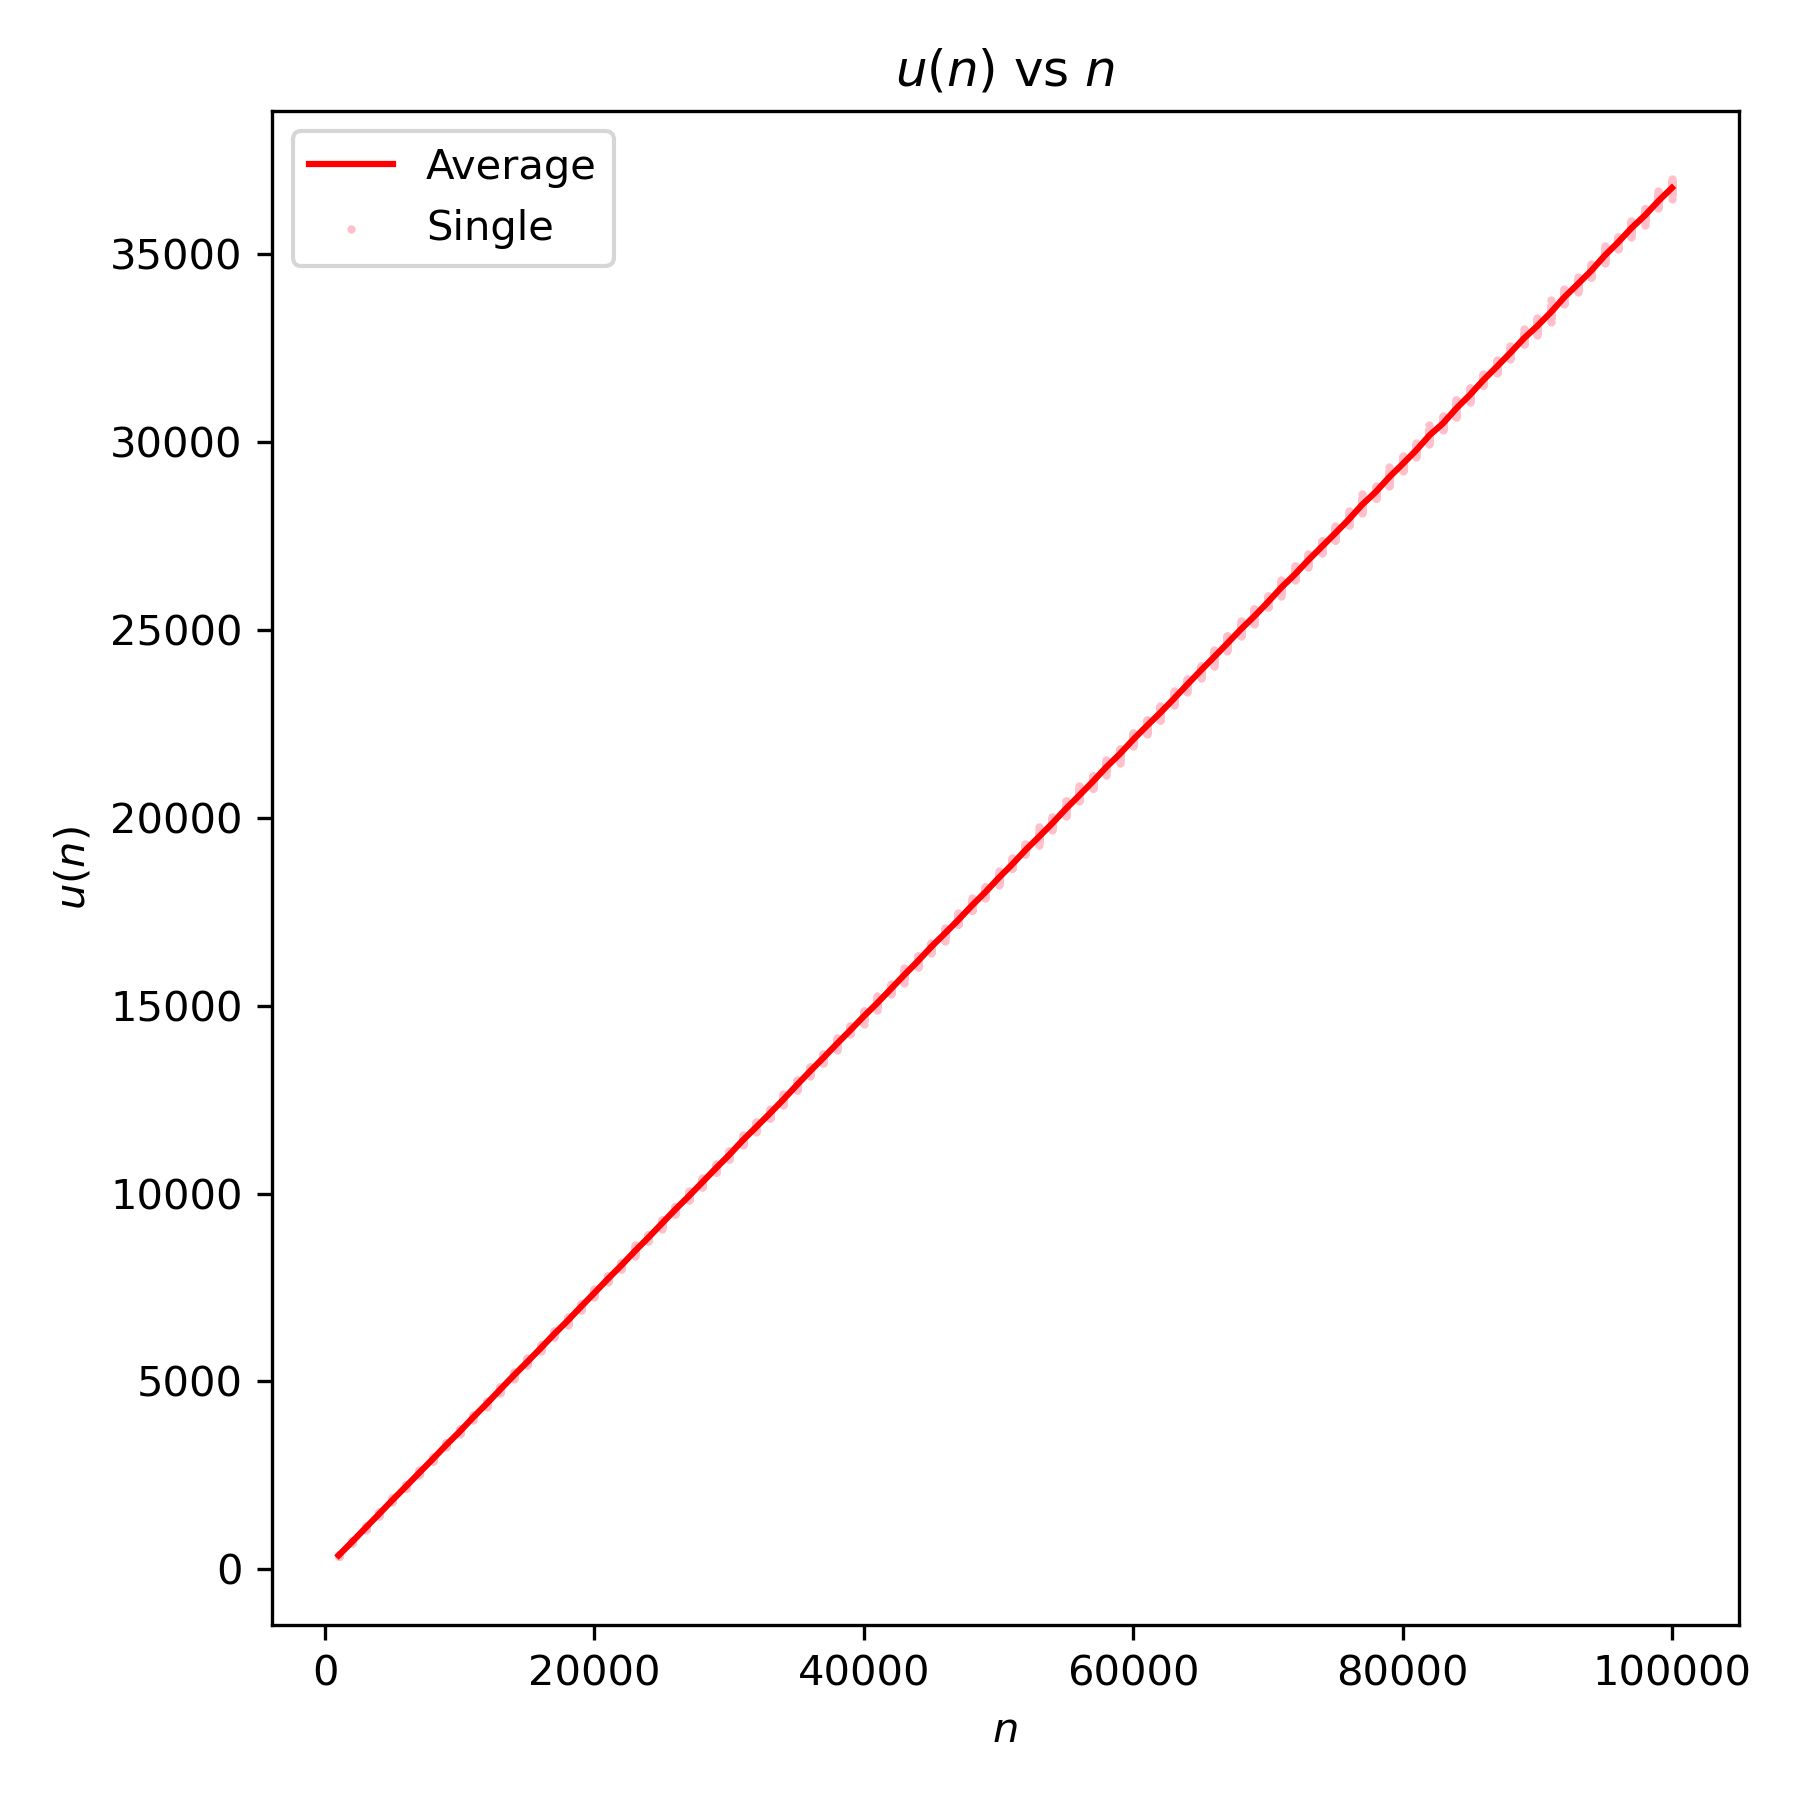
\includegraphics[width=\linewidth]{u_factor_vs_n.png}
        \caption{$u(n)$}
    \end{minipage}
    \begin{minipage}{0.24\textwidth}
        \centering
        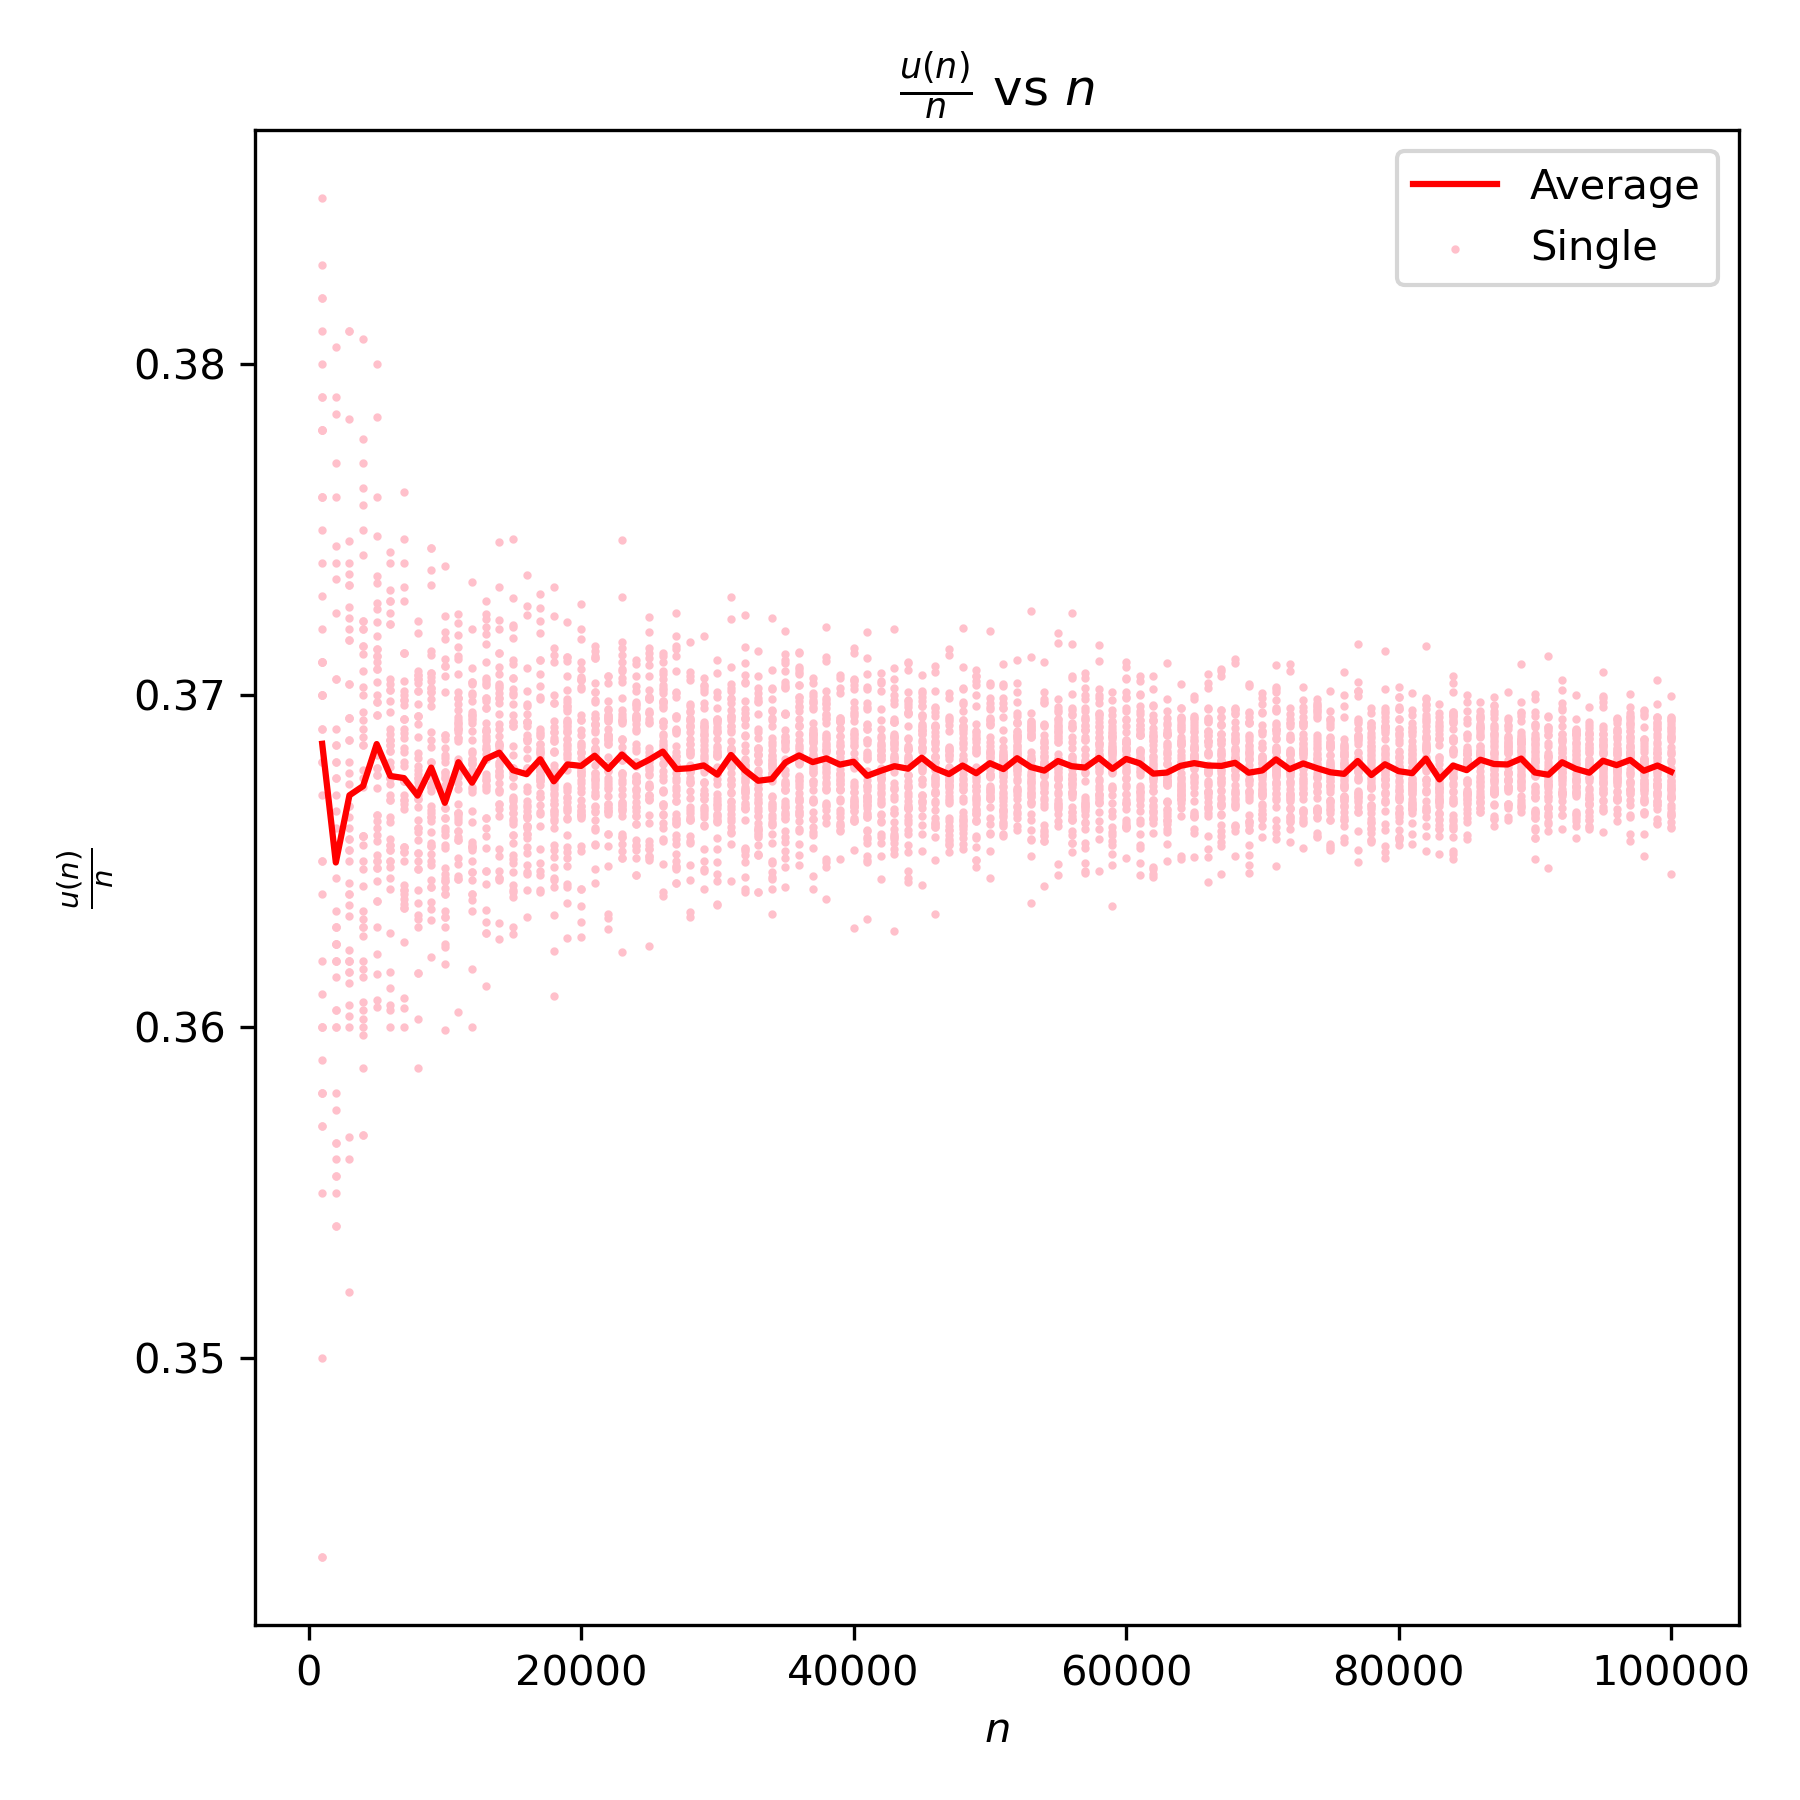
\includegraphics[width=\linewidth]{u_factor_over_n_vs_n.png}
        \caption{$\frac{u(n)}{n}$}
    \end{minipage}
\end{figure}


\subsubsection{Problem Kolekcjonera Kuponów - $C_n$, $\frac{c(n)}{n}$, $\frac{c(n)}{n\ln(n)}$, $\frac{c(n)}{n^2}$}

\begin{figure}[H]
    \centering
    \begin{minipage}{0.24\textwidth}
        \centering
        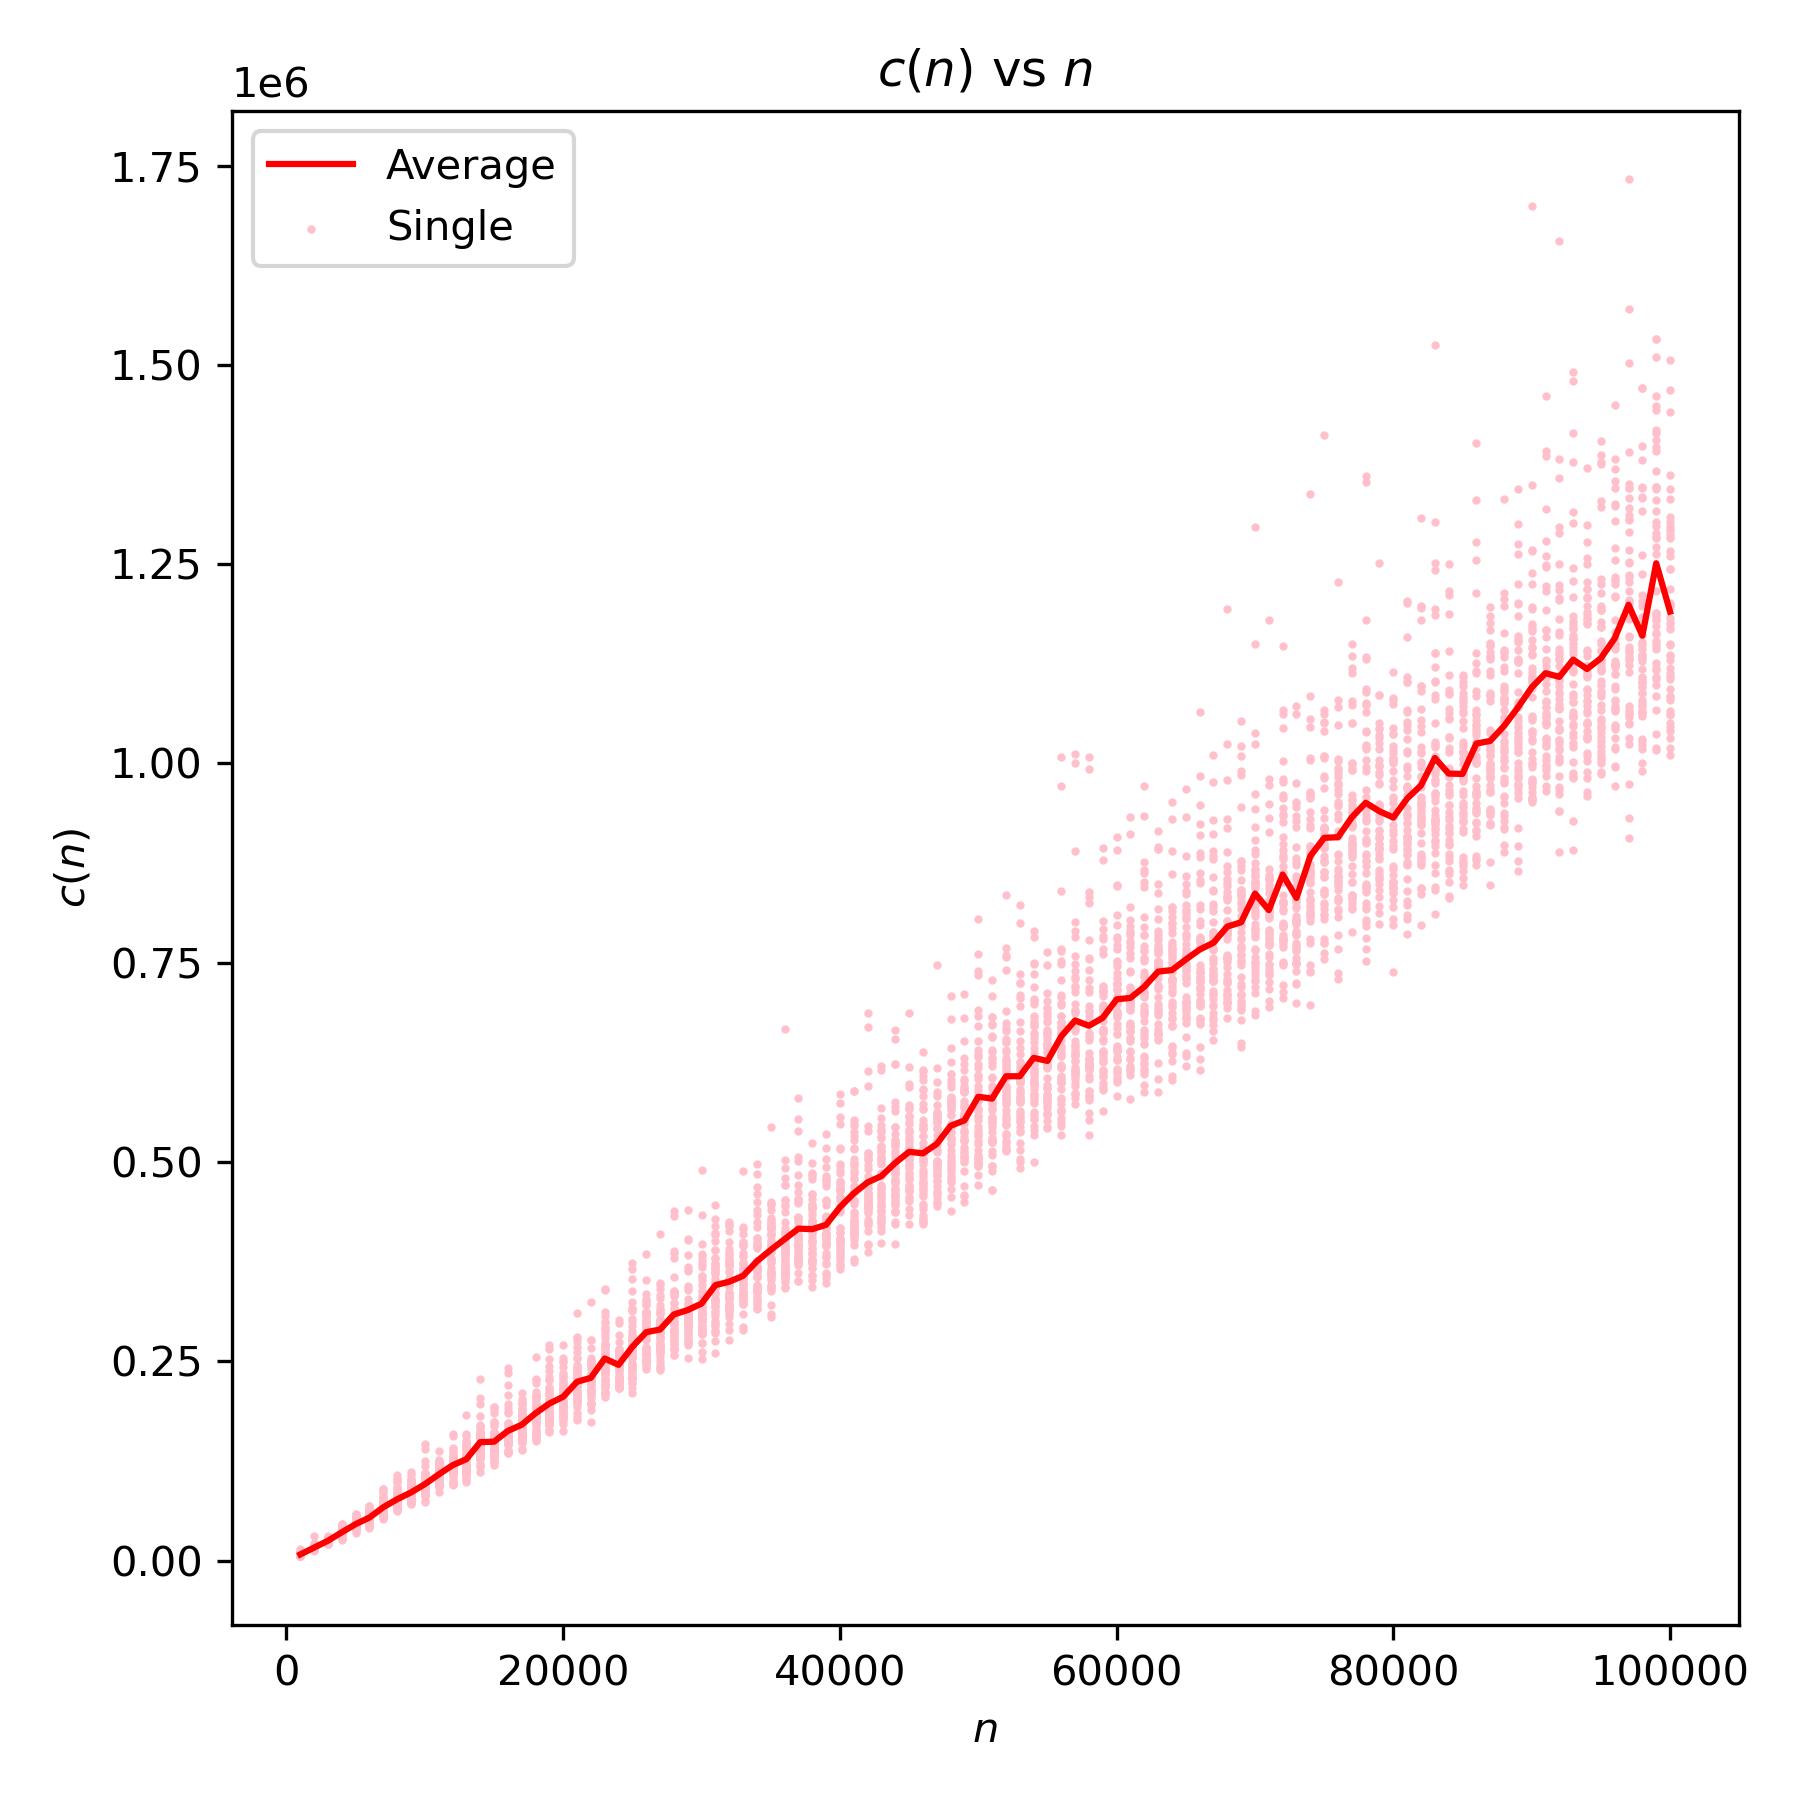
\includegraphics[width=\linewidth]{c_factor_vs_n.png}
        \caption{$C(n)$}
    \end{minipage}
    \begin{minipage}{0.24\textwidth}
        \centering
        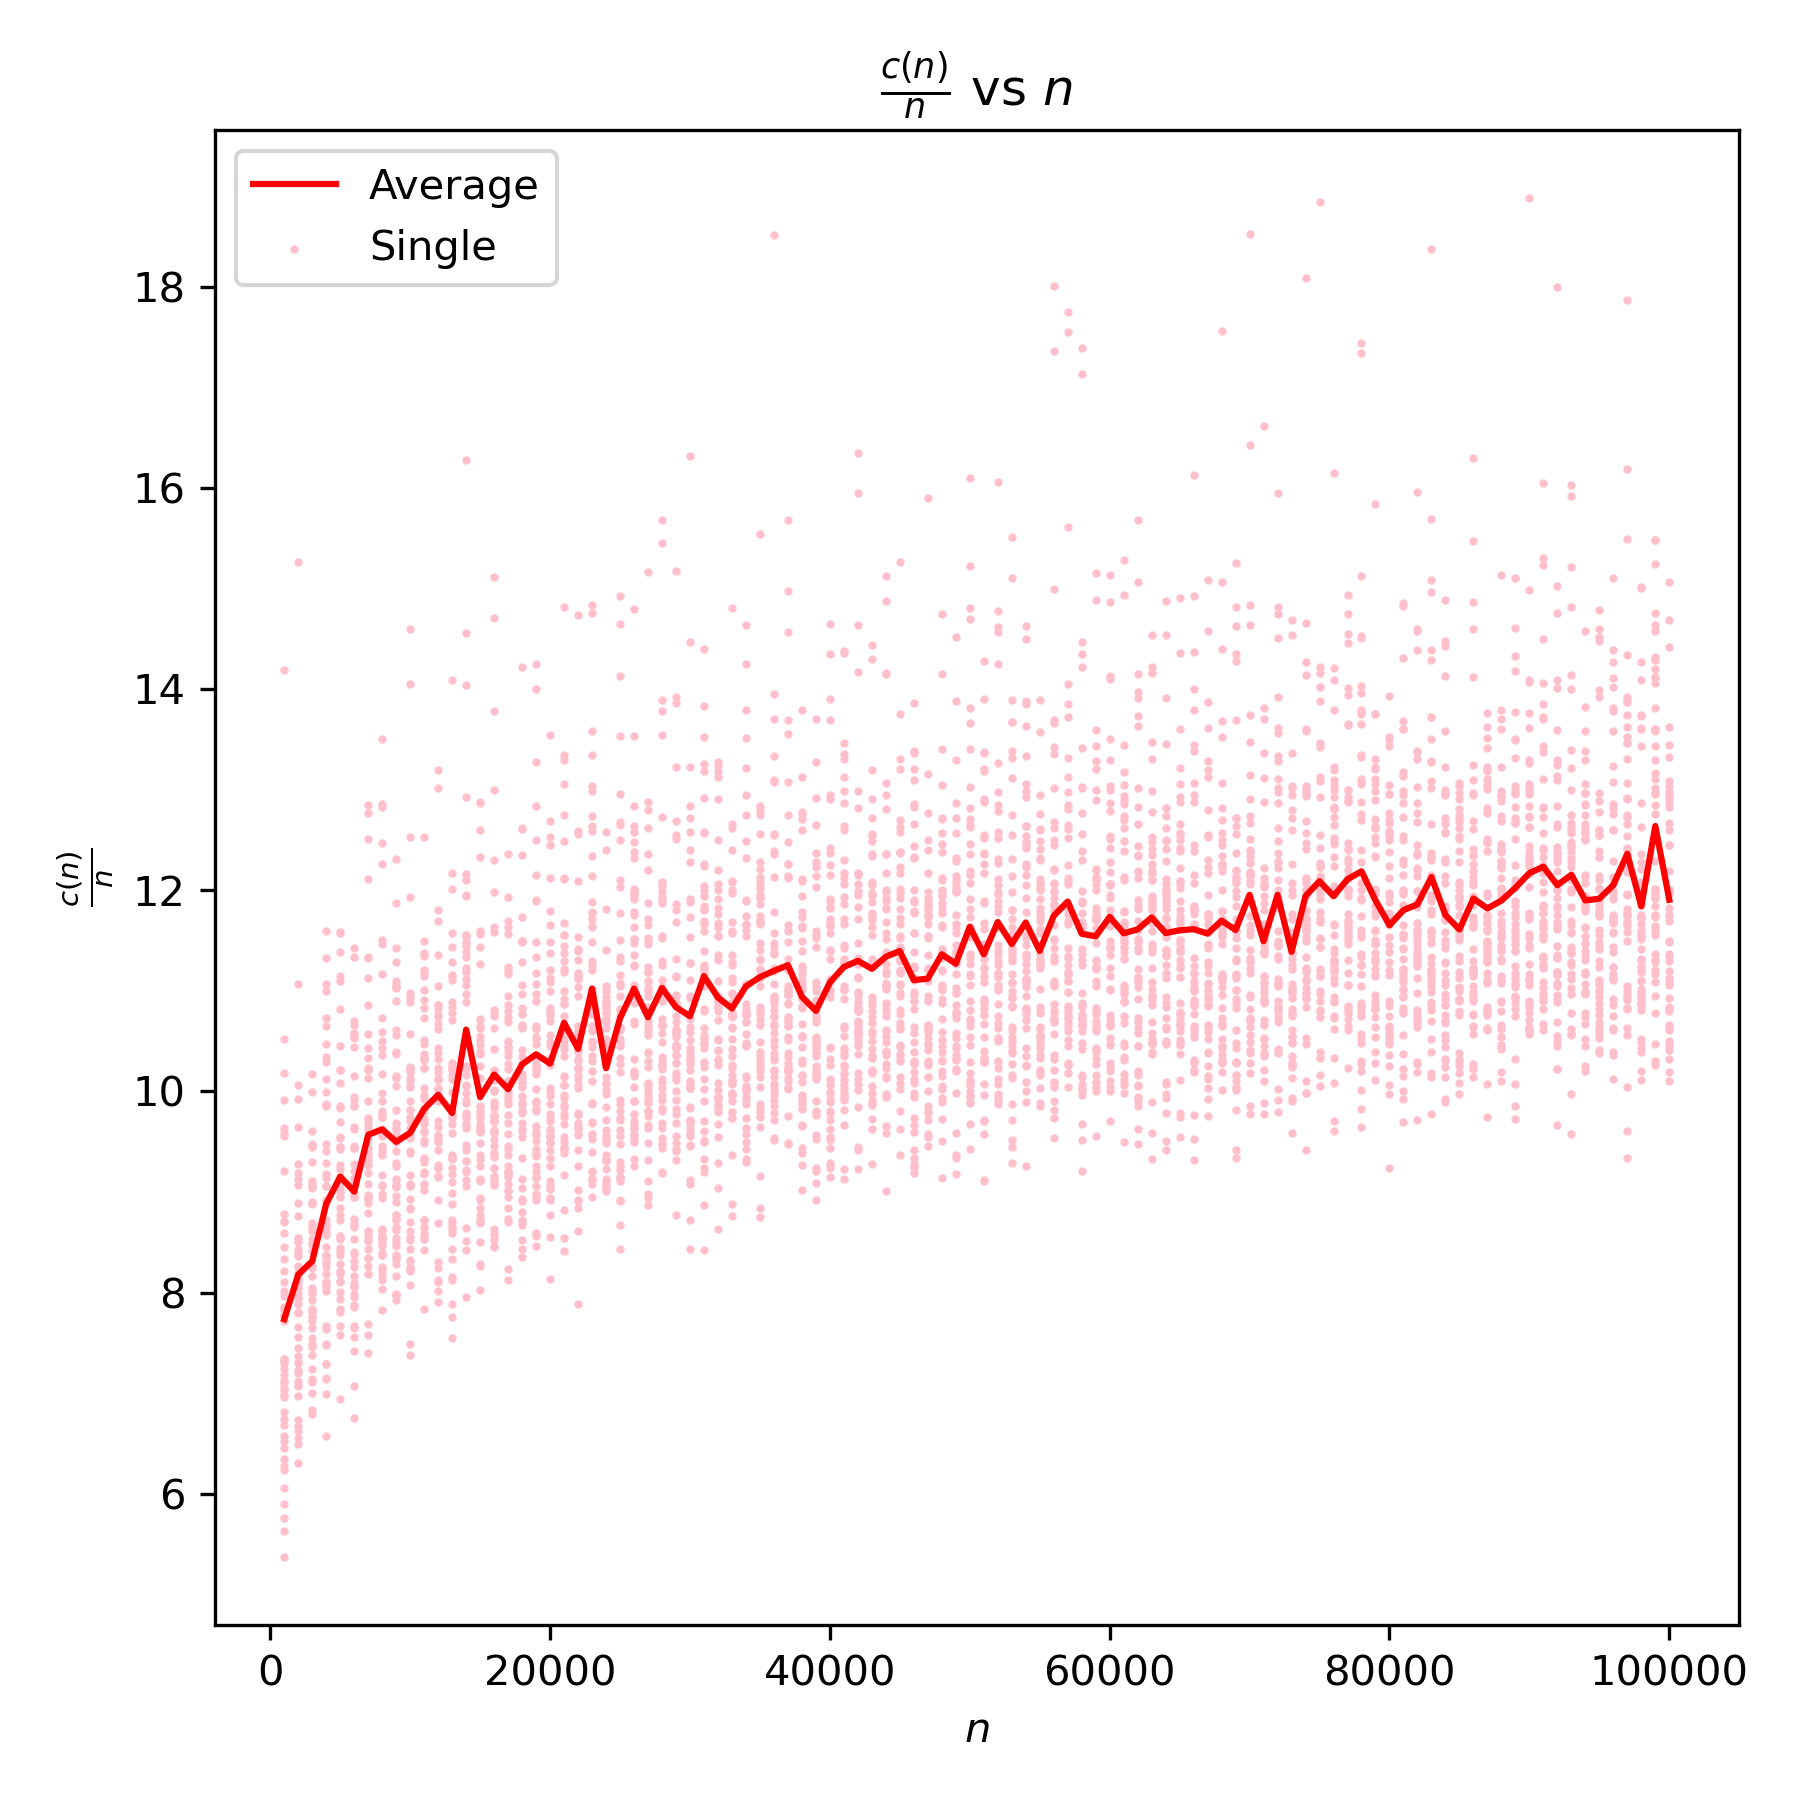
\includegraphics[width=\linewidth]{c_factor_over_n_vs_n.png}
        \caption{$\frac{c(n)}{n}$}
    \end{minipage}
    \begin{minipage}{0.24\textwidth}
        \centering
        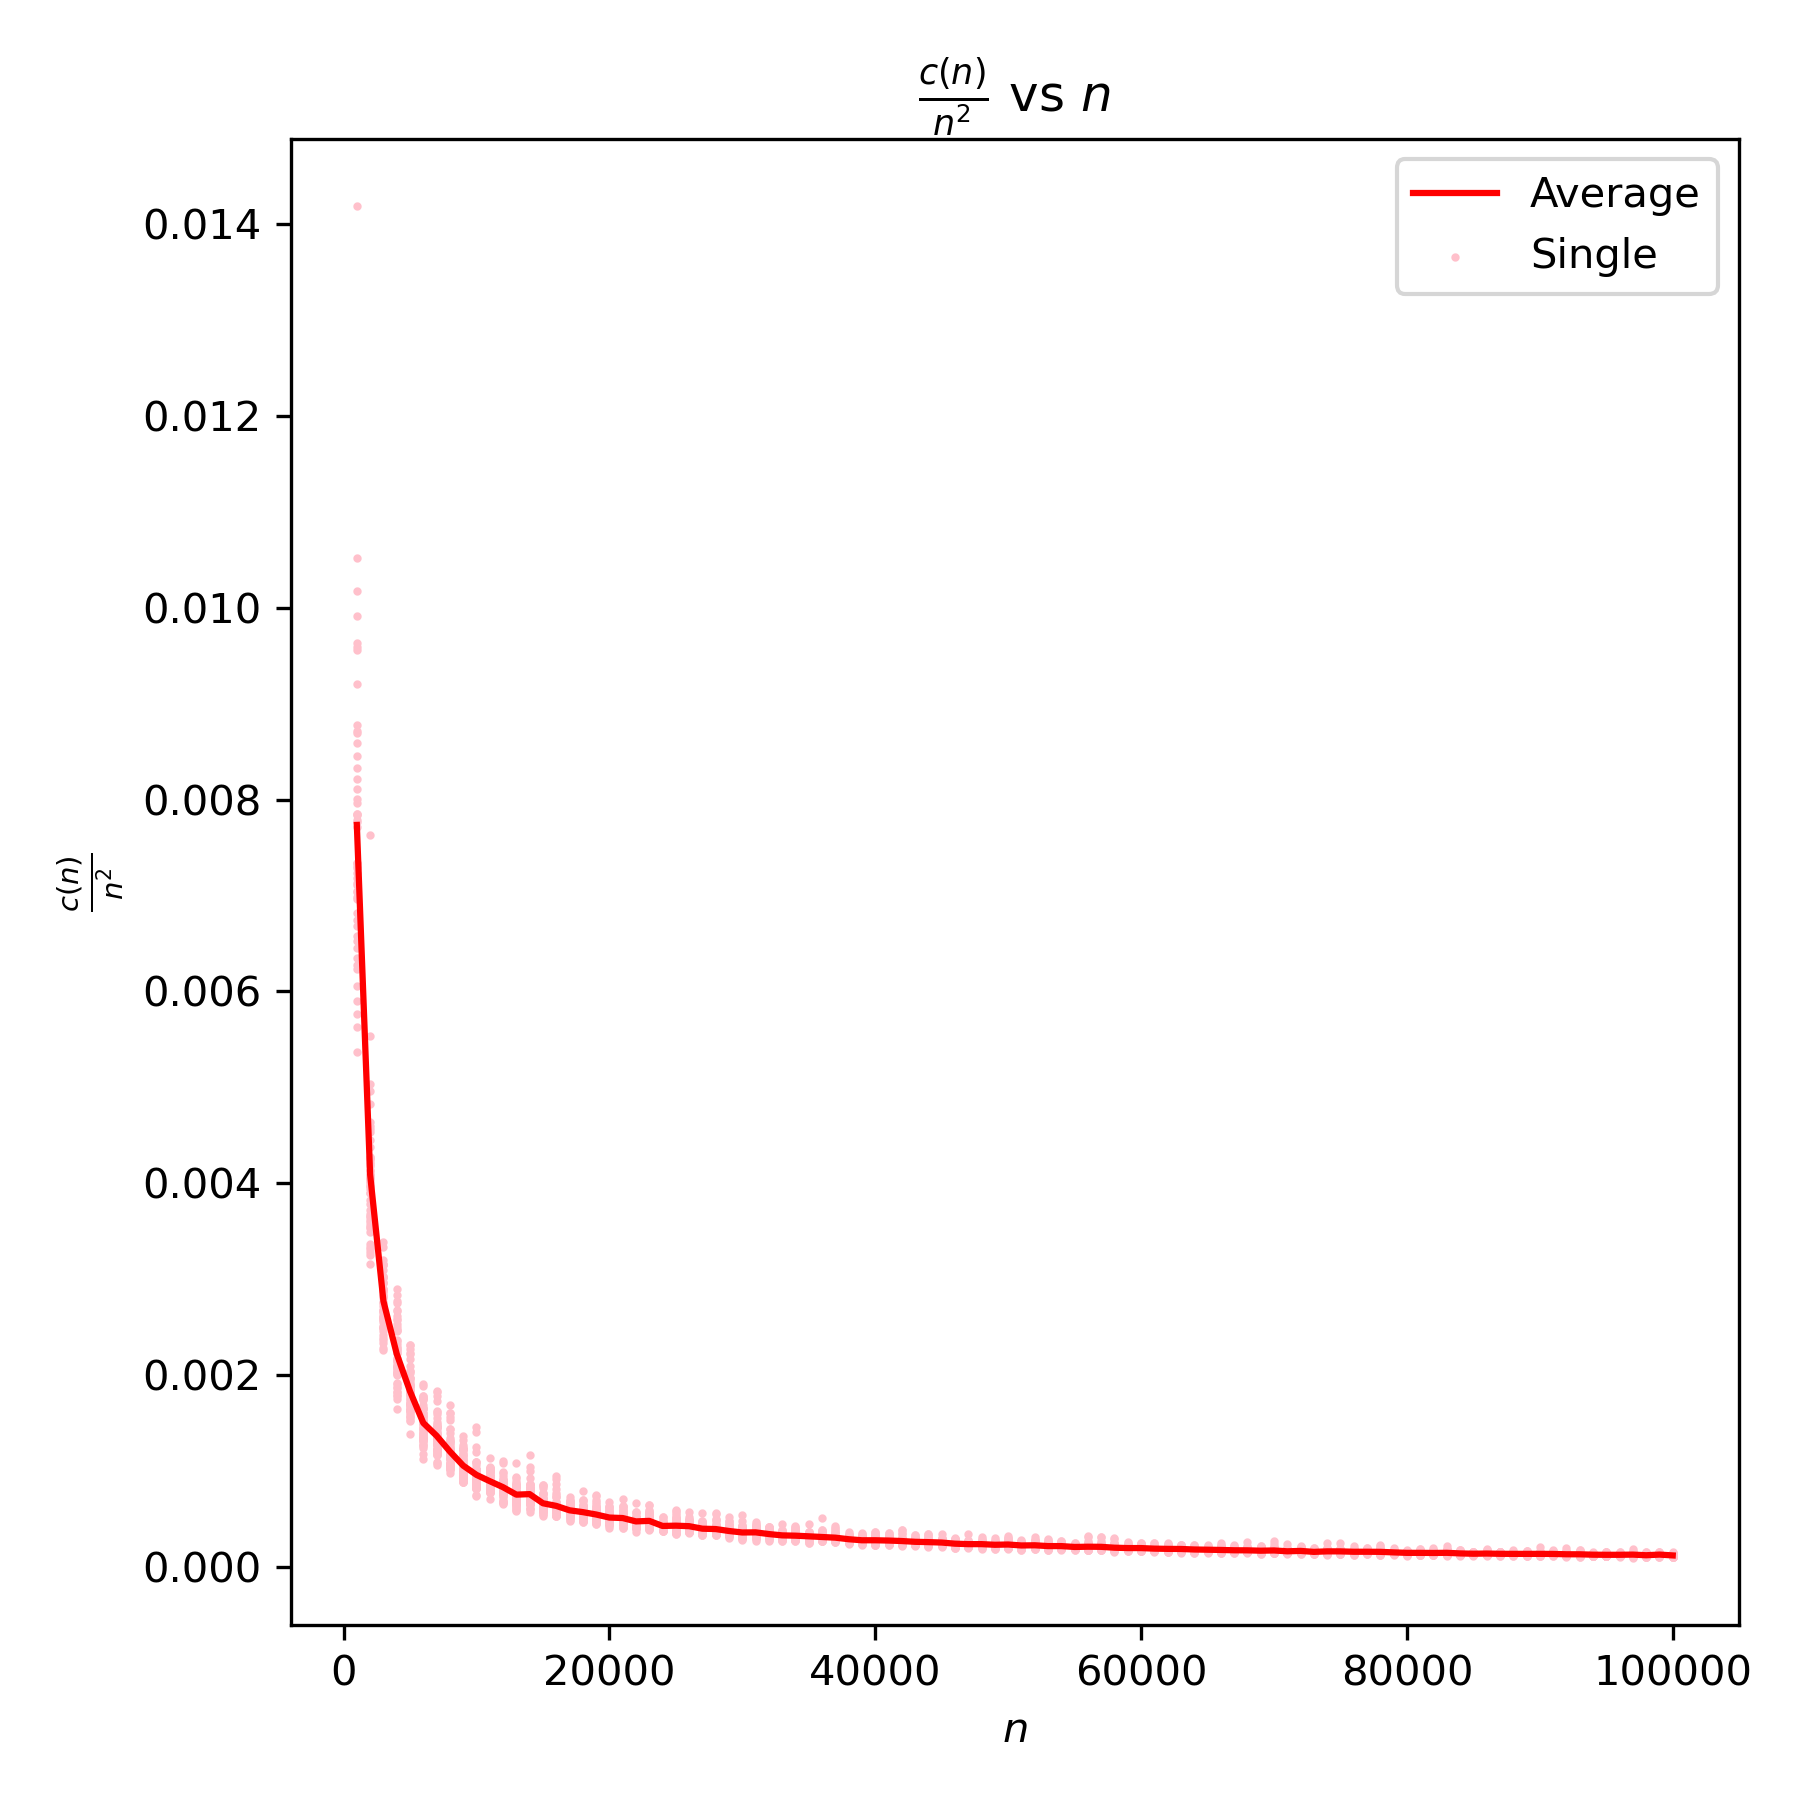
\includegraphics[width=\linewidth]{c_factor_over_n_squared_vs_n.png}
        \caption{$\frac{c(n)}{n^2}$}
    \end{minipage}
        \begin{minipage}{0.24\textwidth}
        \centering
        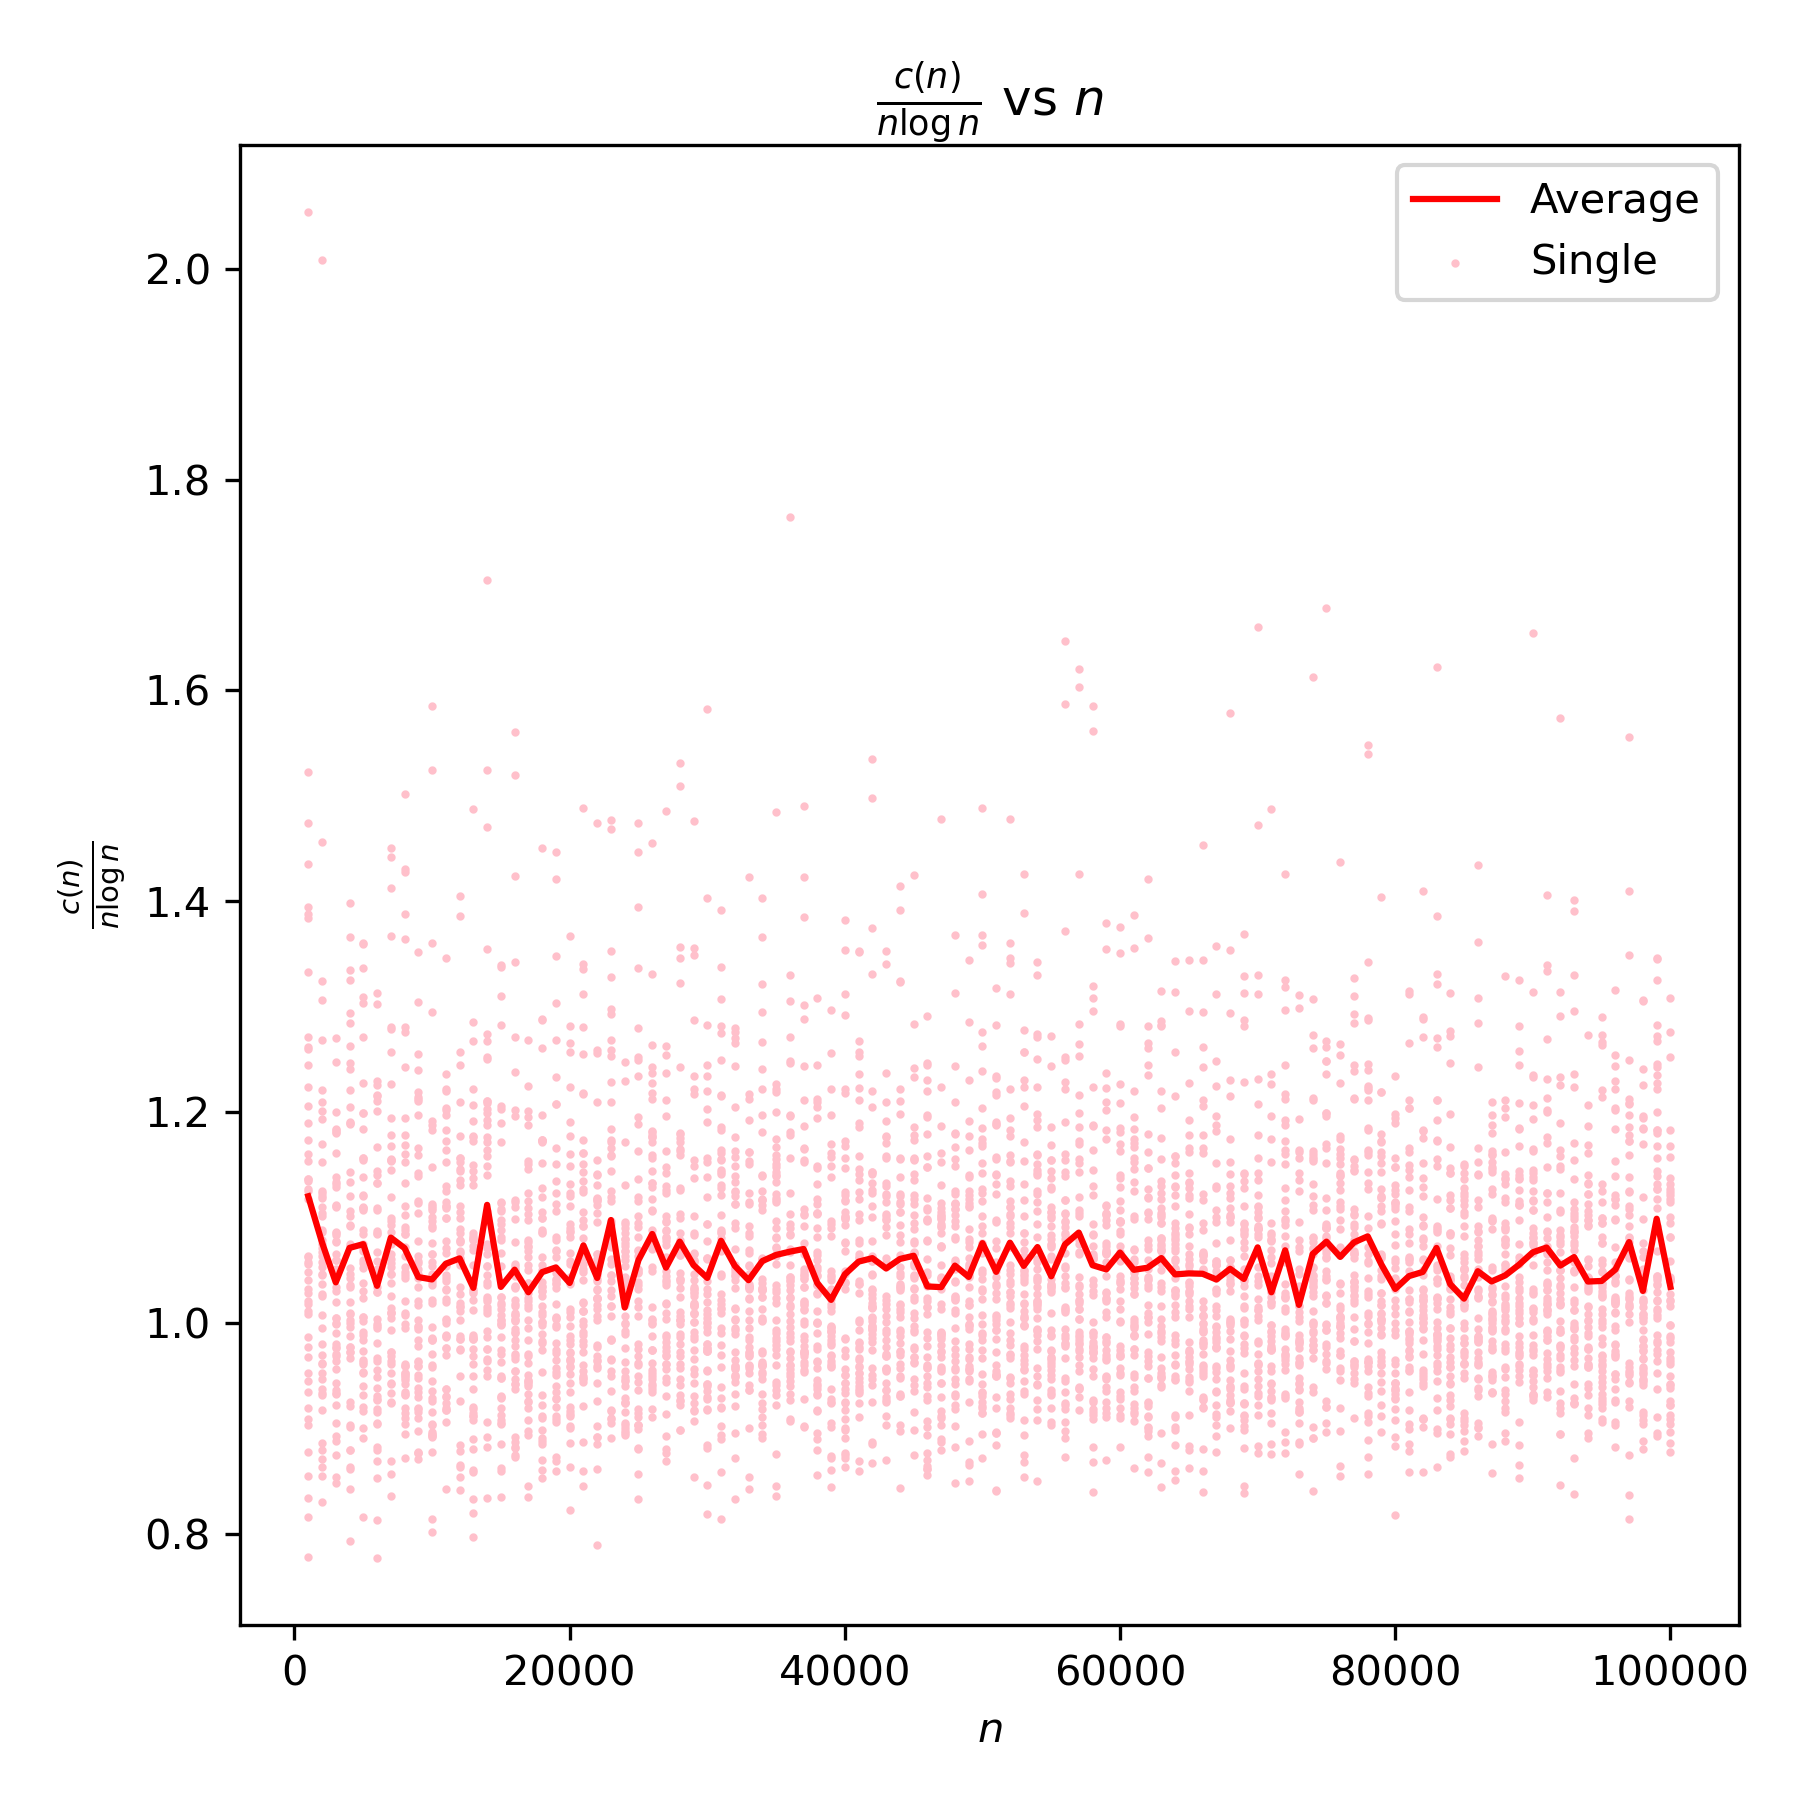
\includegraphics[width=\linewidth]{c_factor_over_n_log_n_vs_n.png}
        \caption{$\frac{c(n)}{n \log(n)}$}
    \end{minipage}
\end{figure}


\subsubsection{Problem Kolekcjonera Dwóch Kuponów - $D_n$, $\frac{d(n)}{n}$, $\frac{d(n)}{n\ln(n)}$, $\frac{d(n)}{n^2}$}

\begin{figure}[H]
    \centering
    \begin{minipage}{0.24\textwidth}
        \centering
        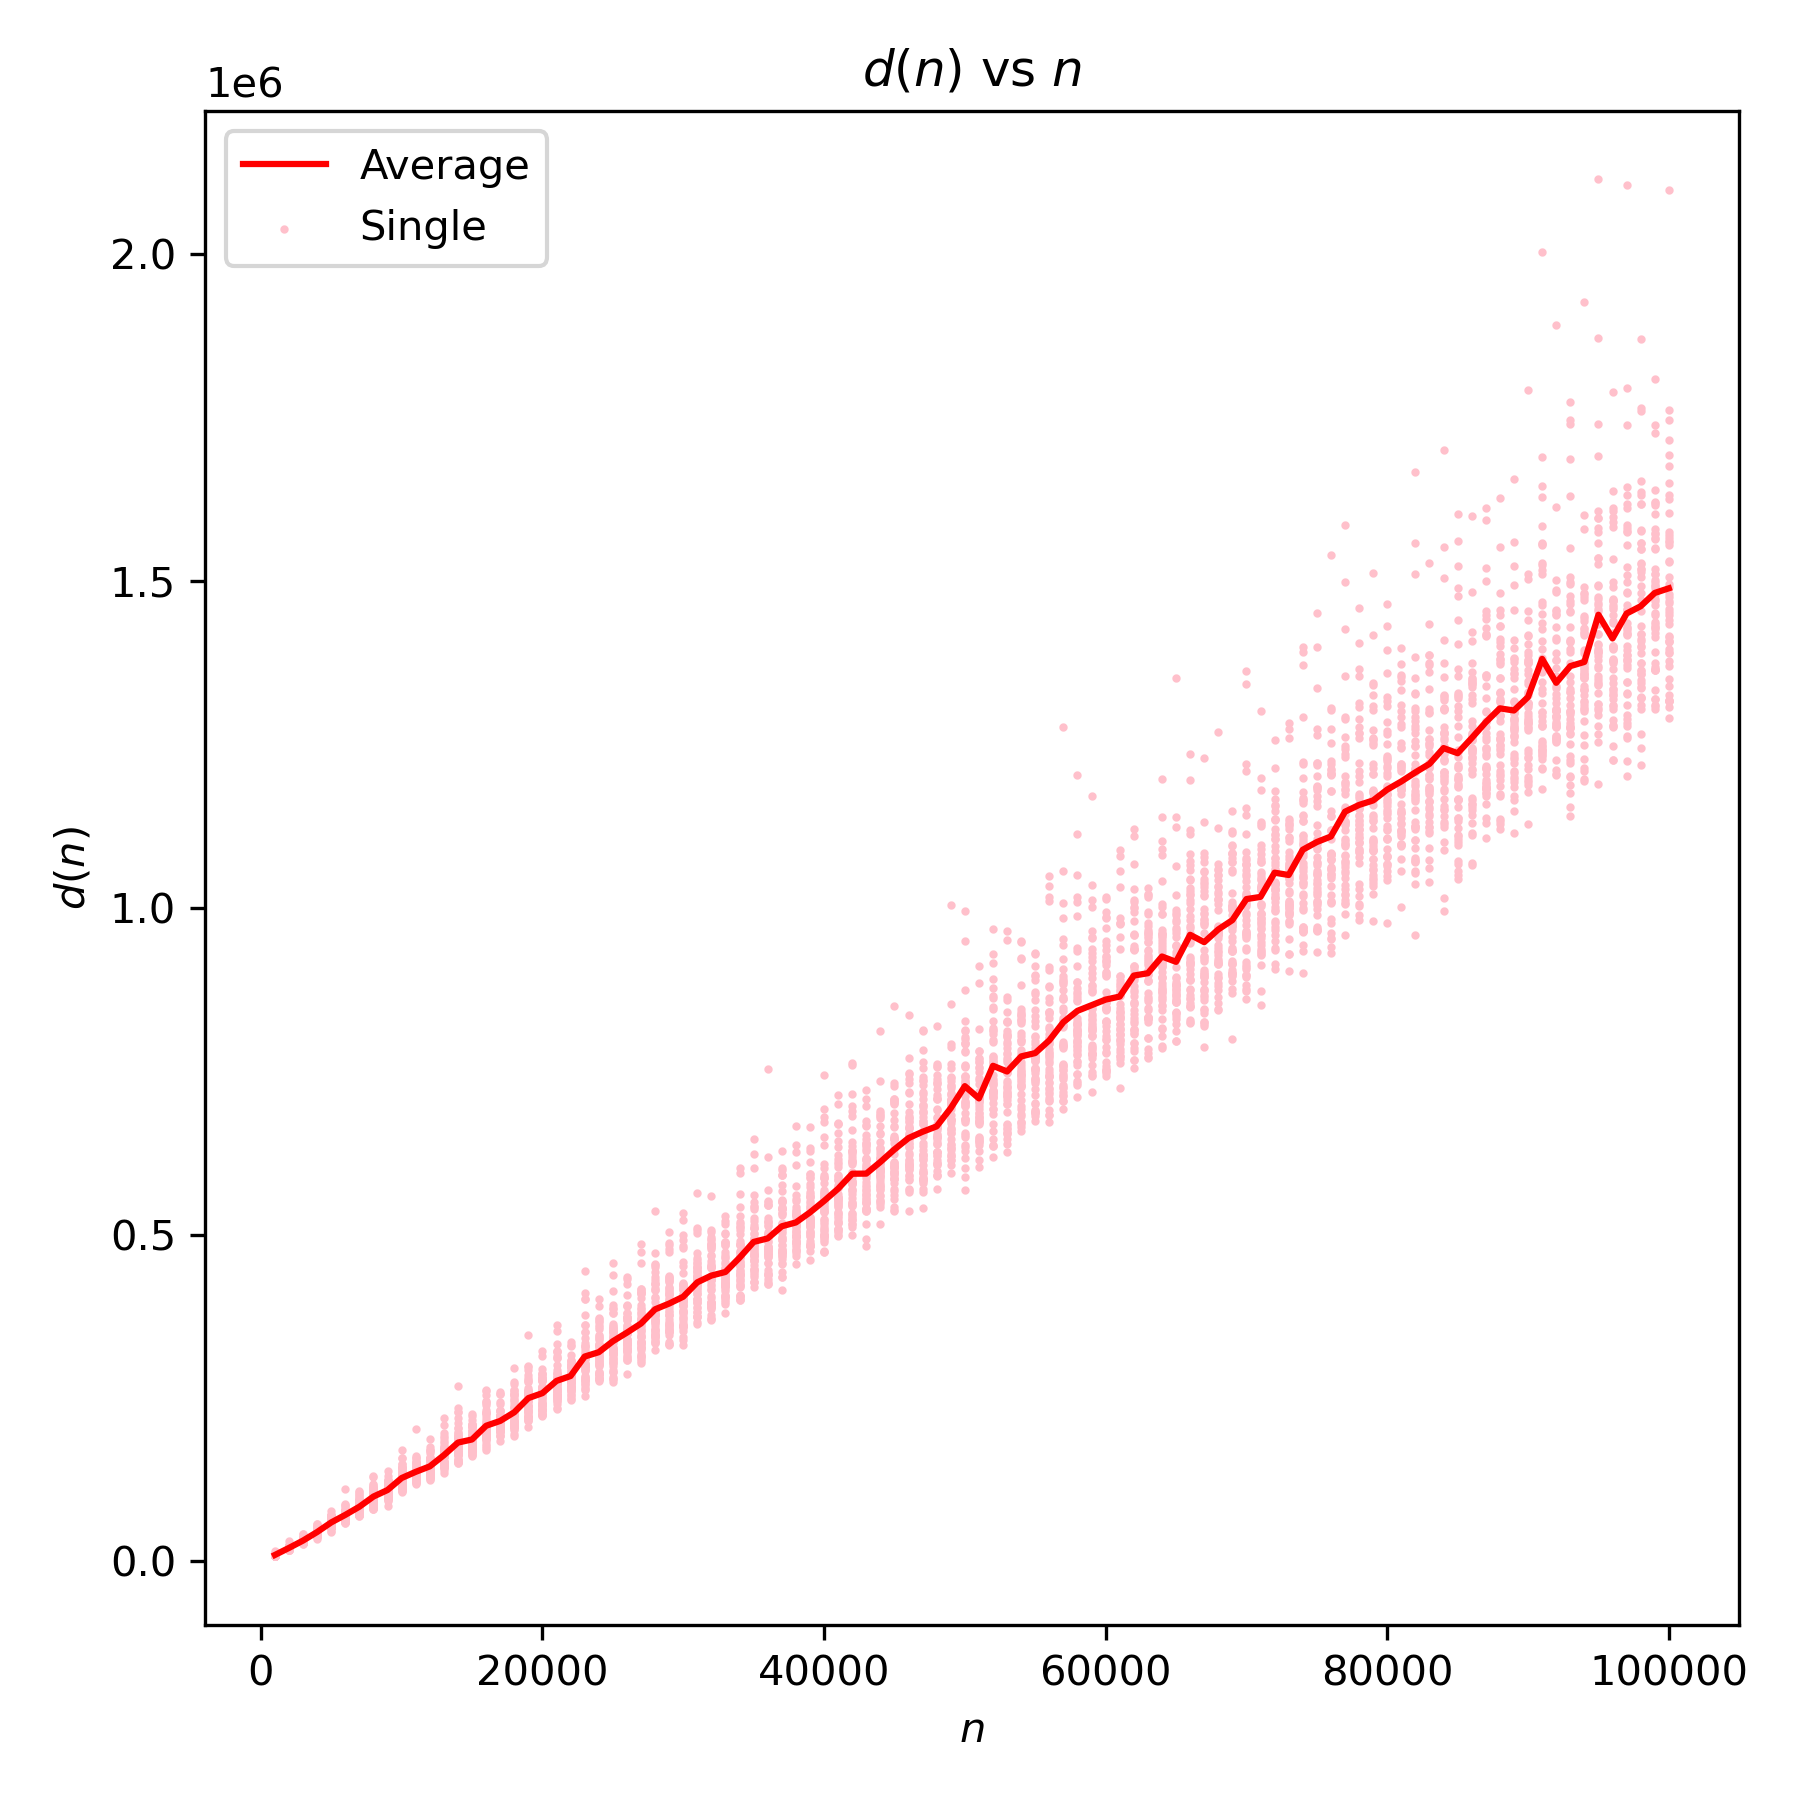
\includegraphics[width=\linewidth]{d_factor_vs_n.png}
        \caption{$D(n)$}
    \end{minipage}
    \begin{minipage}{0.24\textwidth}
        \centering
        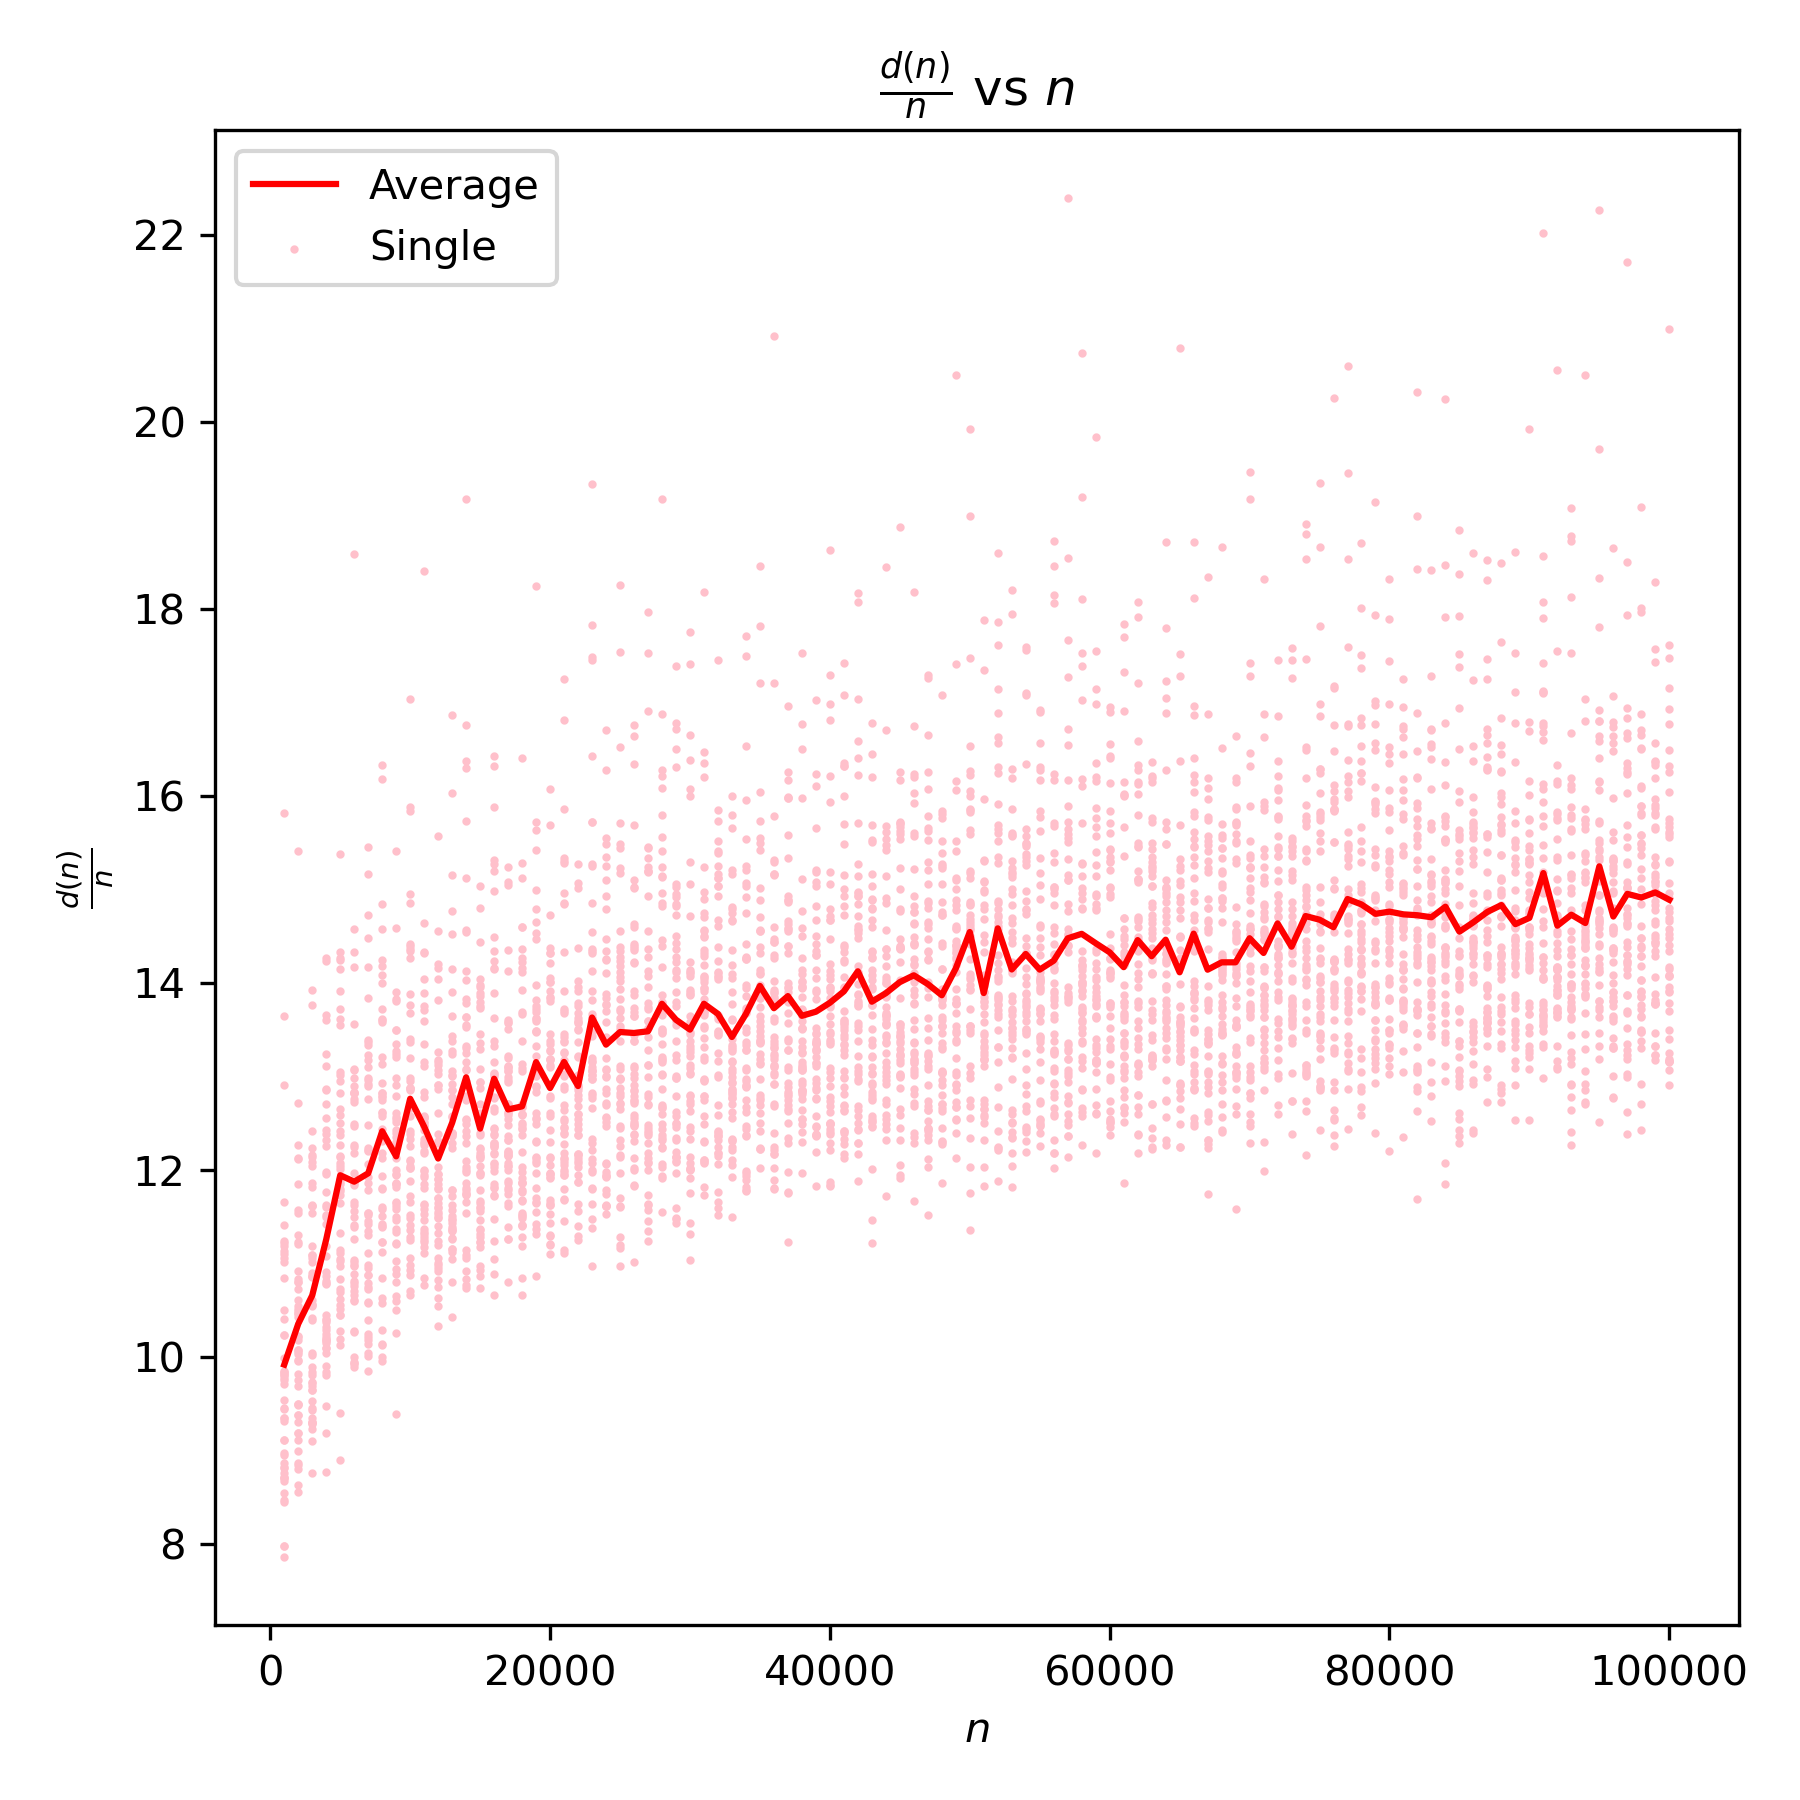
\includegraphics[width=\linewidth]{d_factor_over_n_vs_n.png}
        \caption{$\frac{d(n)}{n}$}
    \end{minipage}
    \begin{minipage}{0.24\textwidth}
        \centering
        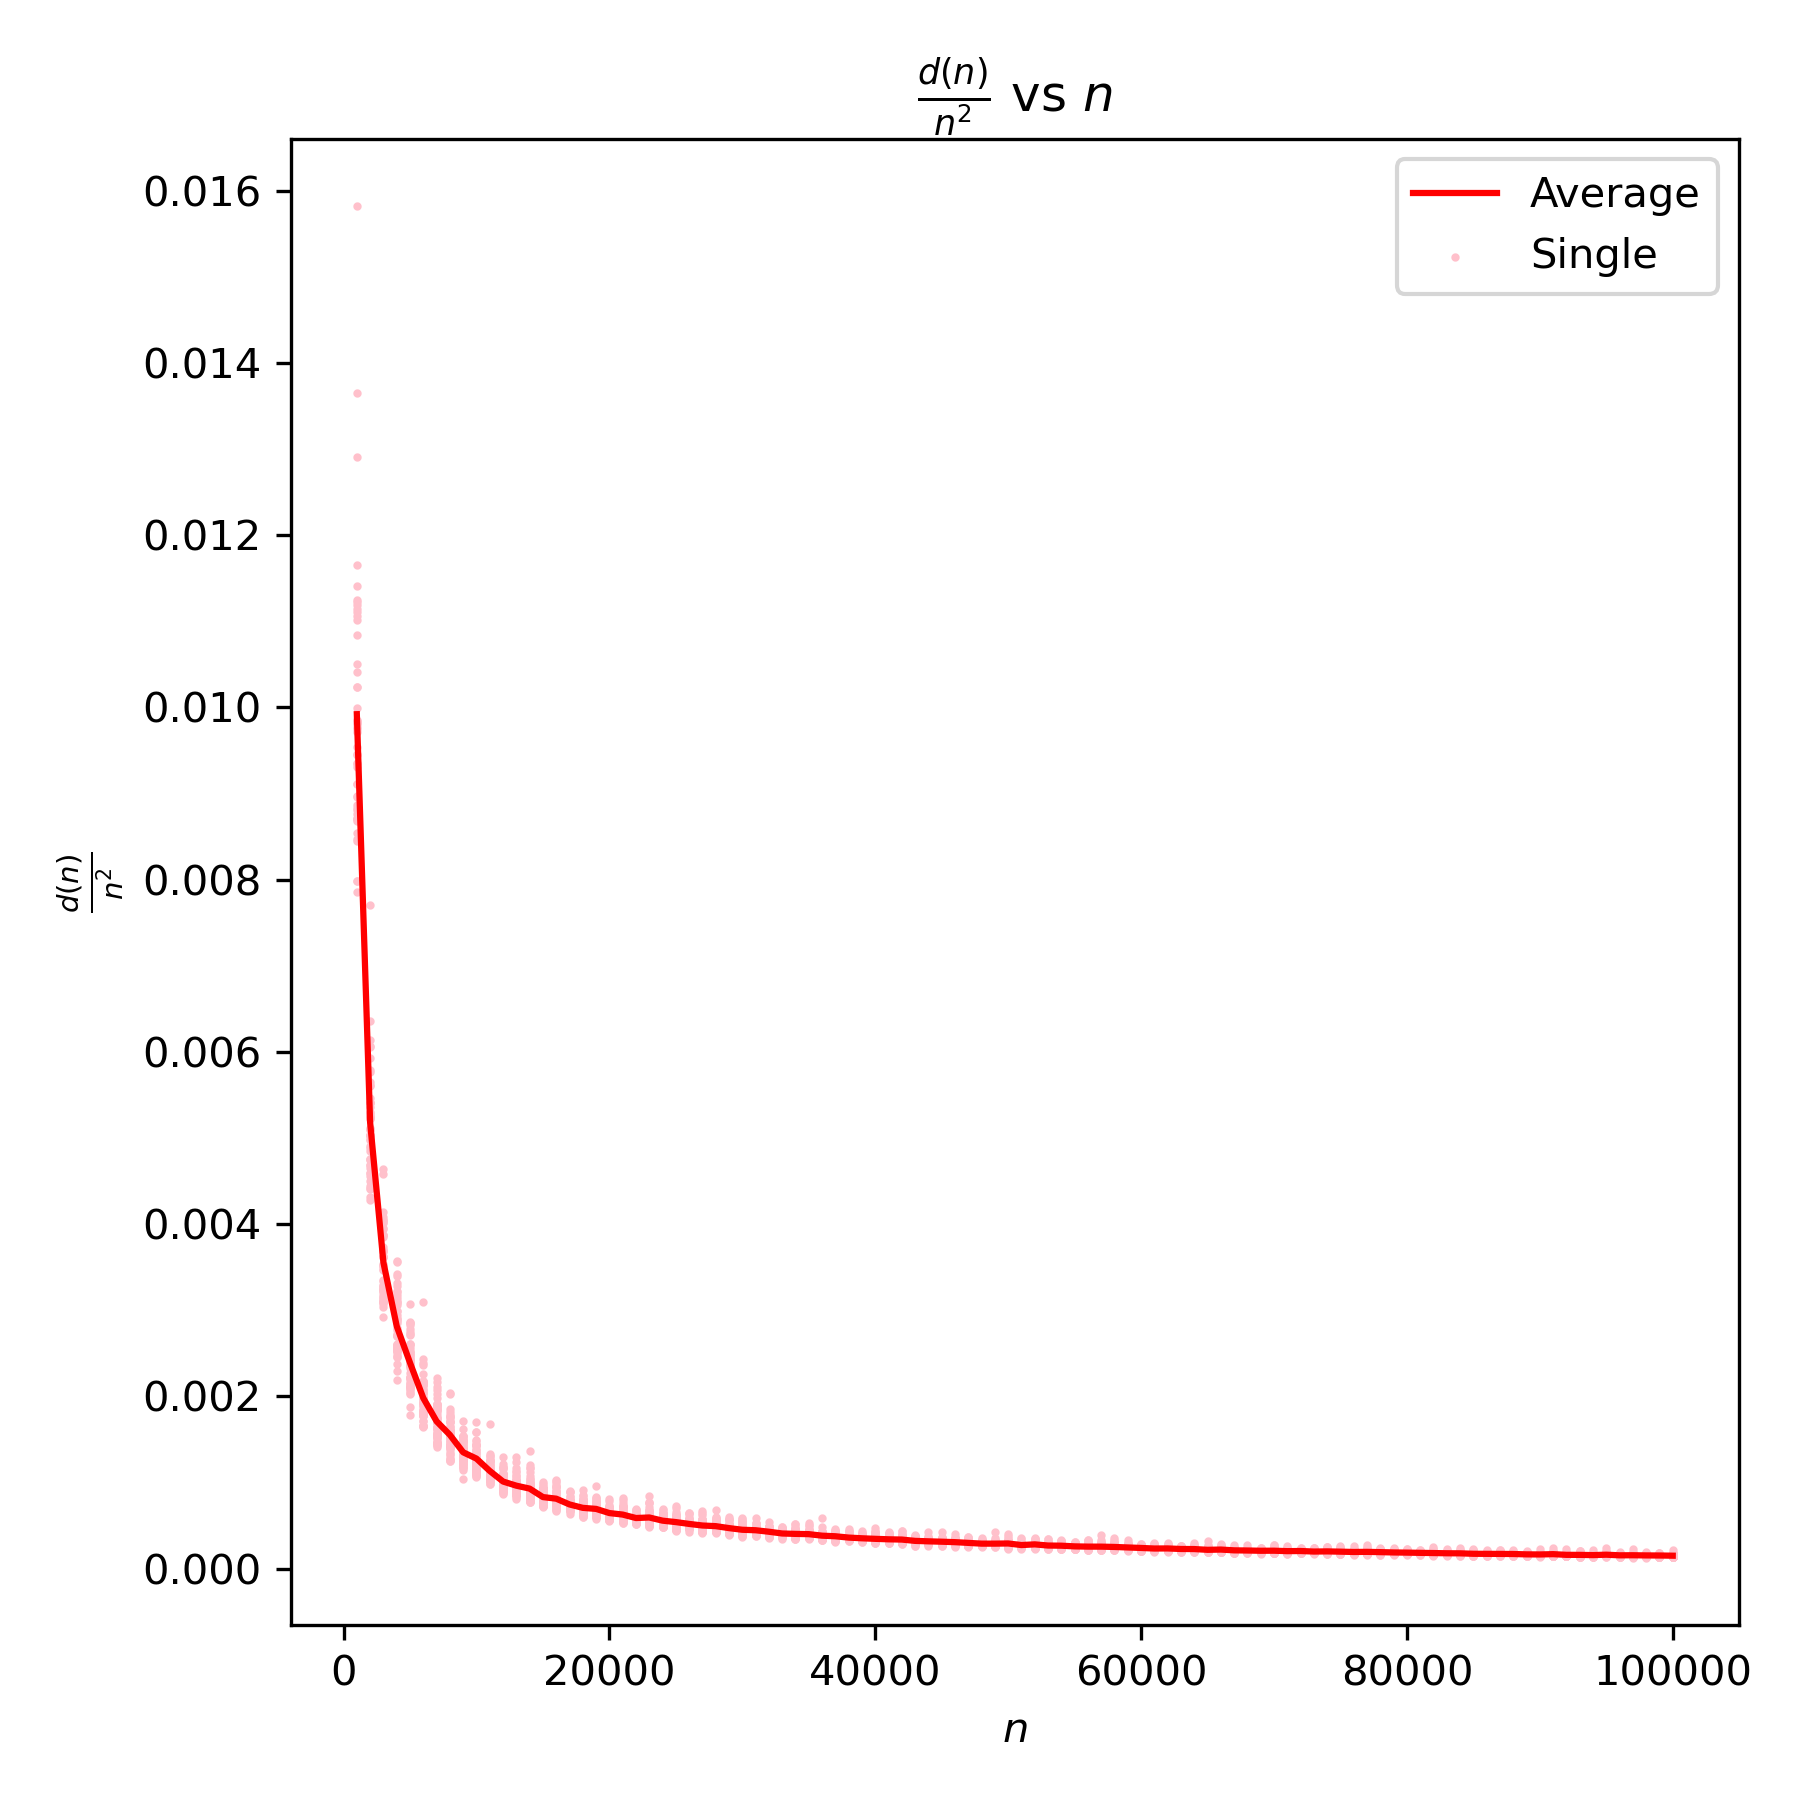
\includegraphics[width=\linewidth]{d_factor_over_n_squared_vs_n.png}
        \caption{$\frac{d(n)}{n^2}$}
    \end{minipage}
    \begin{minipage}{0.24\textwidth}
        \centering
        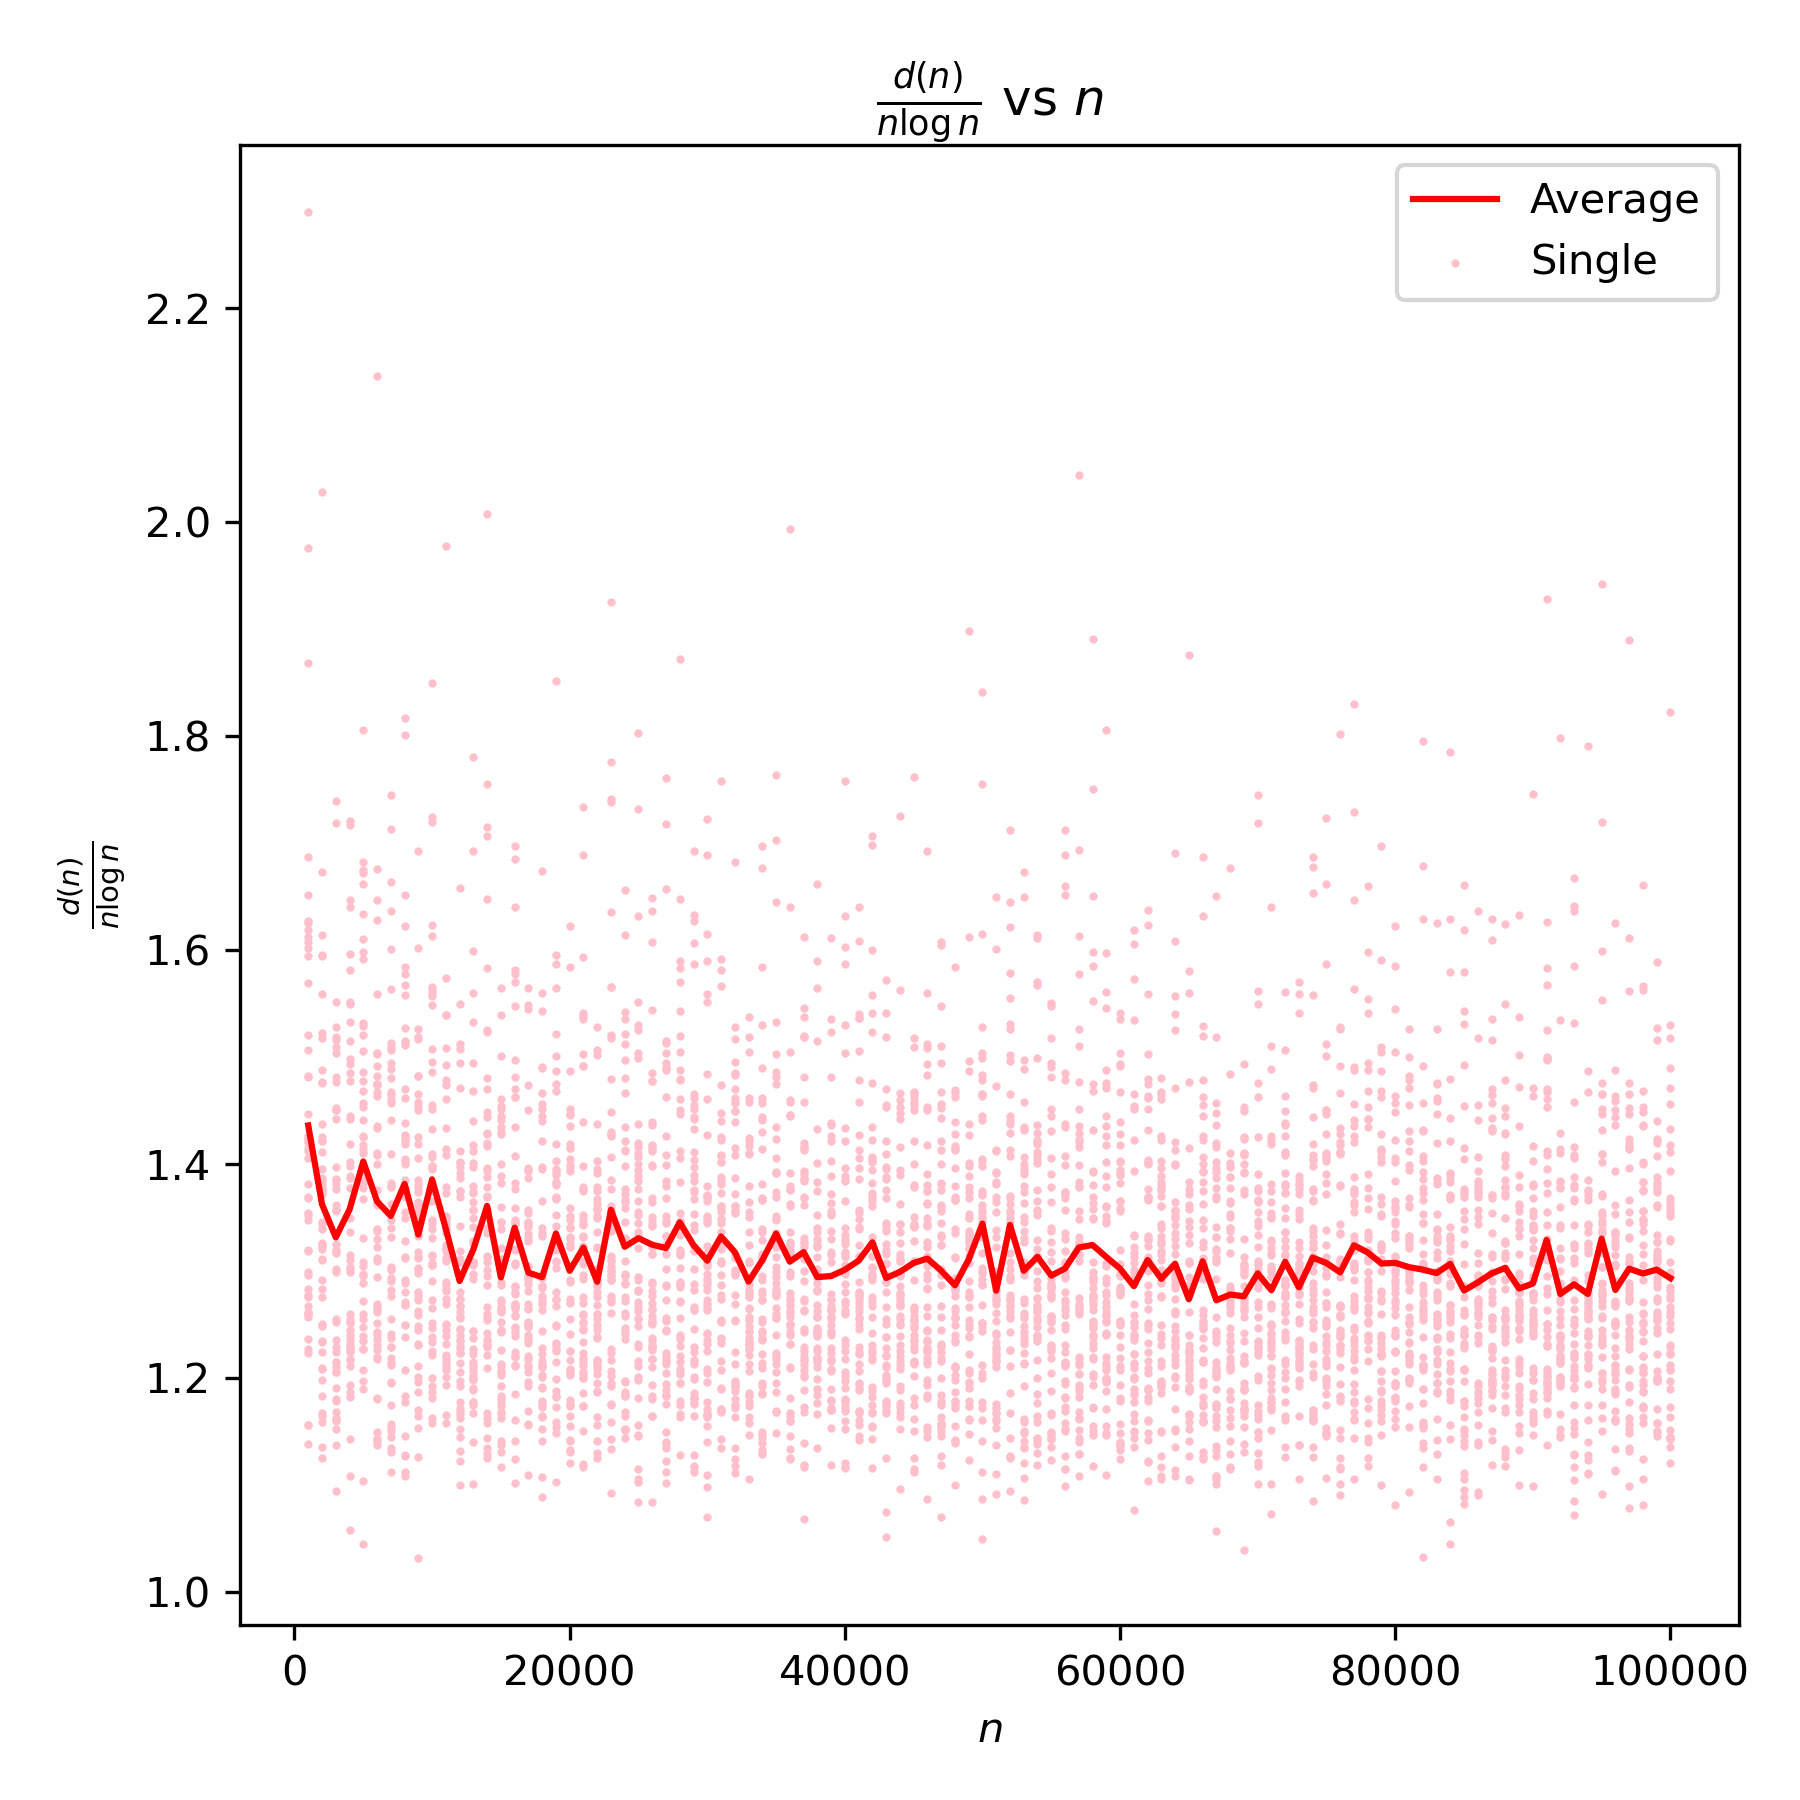
\includegraphics[width=\linewidth]{d_factor_over_n_log_n_vs_n.png}
        \caption{$\frac{d(n)}{n \log(n)}$}
    \end{minipage}
\end{figure}


\subsubsection{Różnica dwóch powyższych - $R_n=D(n)-C(n)$, $\frac{r(n)}{n}$, $\frac{r(n)}{n\ln(n)}$, $\frac{r(n)}{n\ln(\ln(n)))}$}

\begin{figure}[H]
    \centering
        \begin{minipage}{0.24\textwidth}
        \centering
        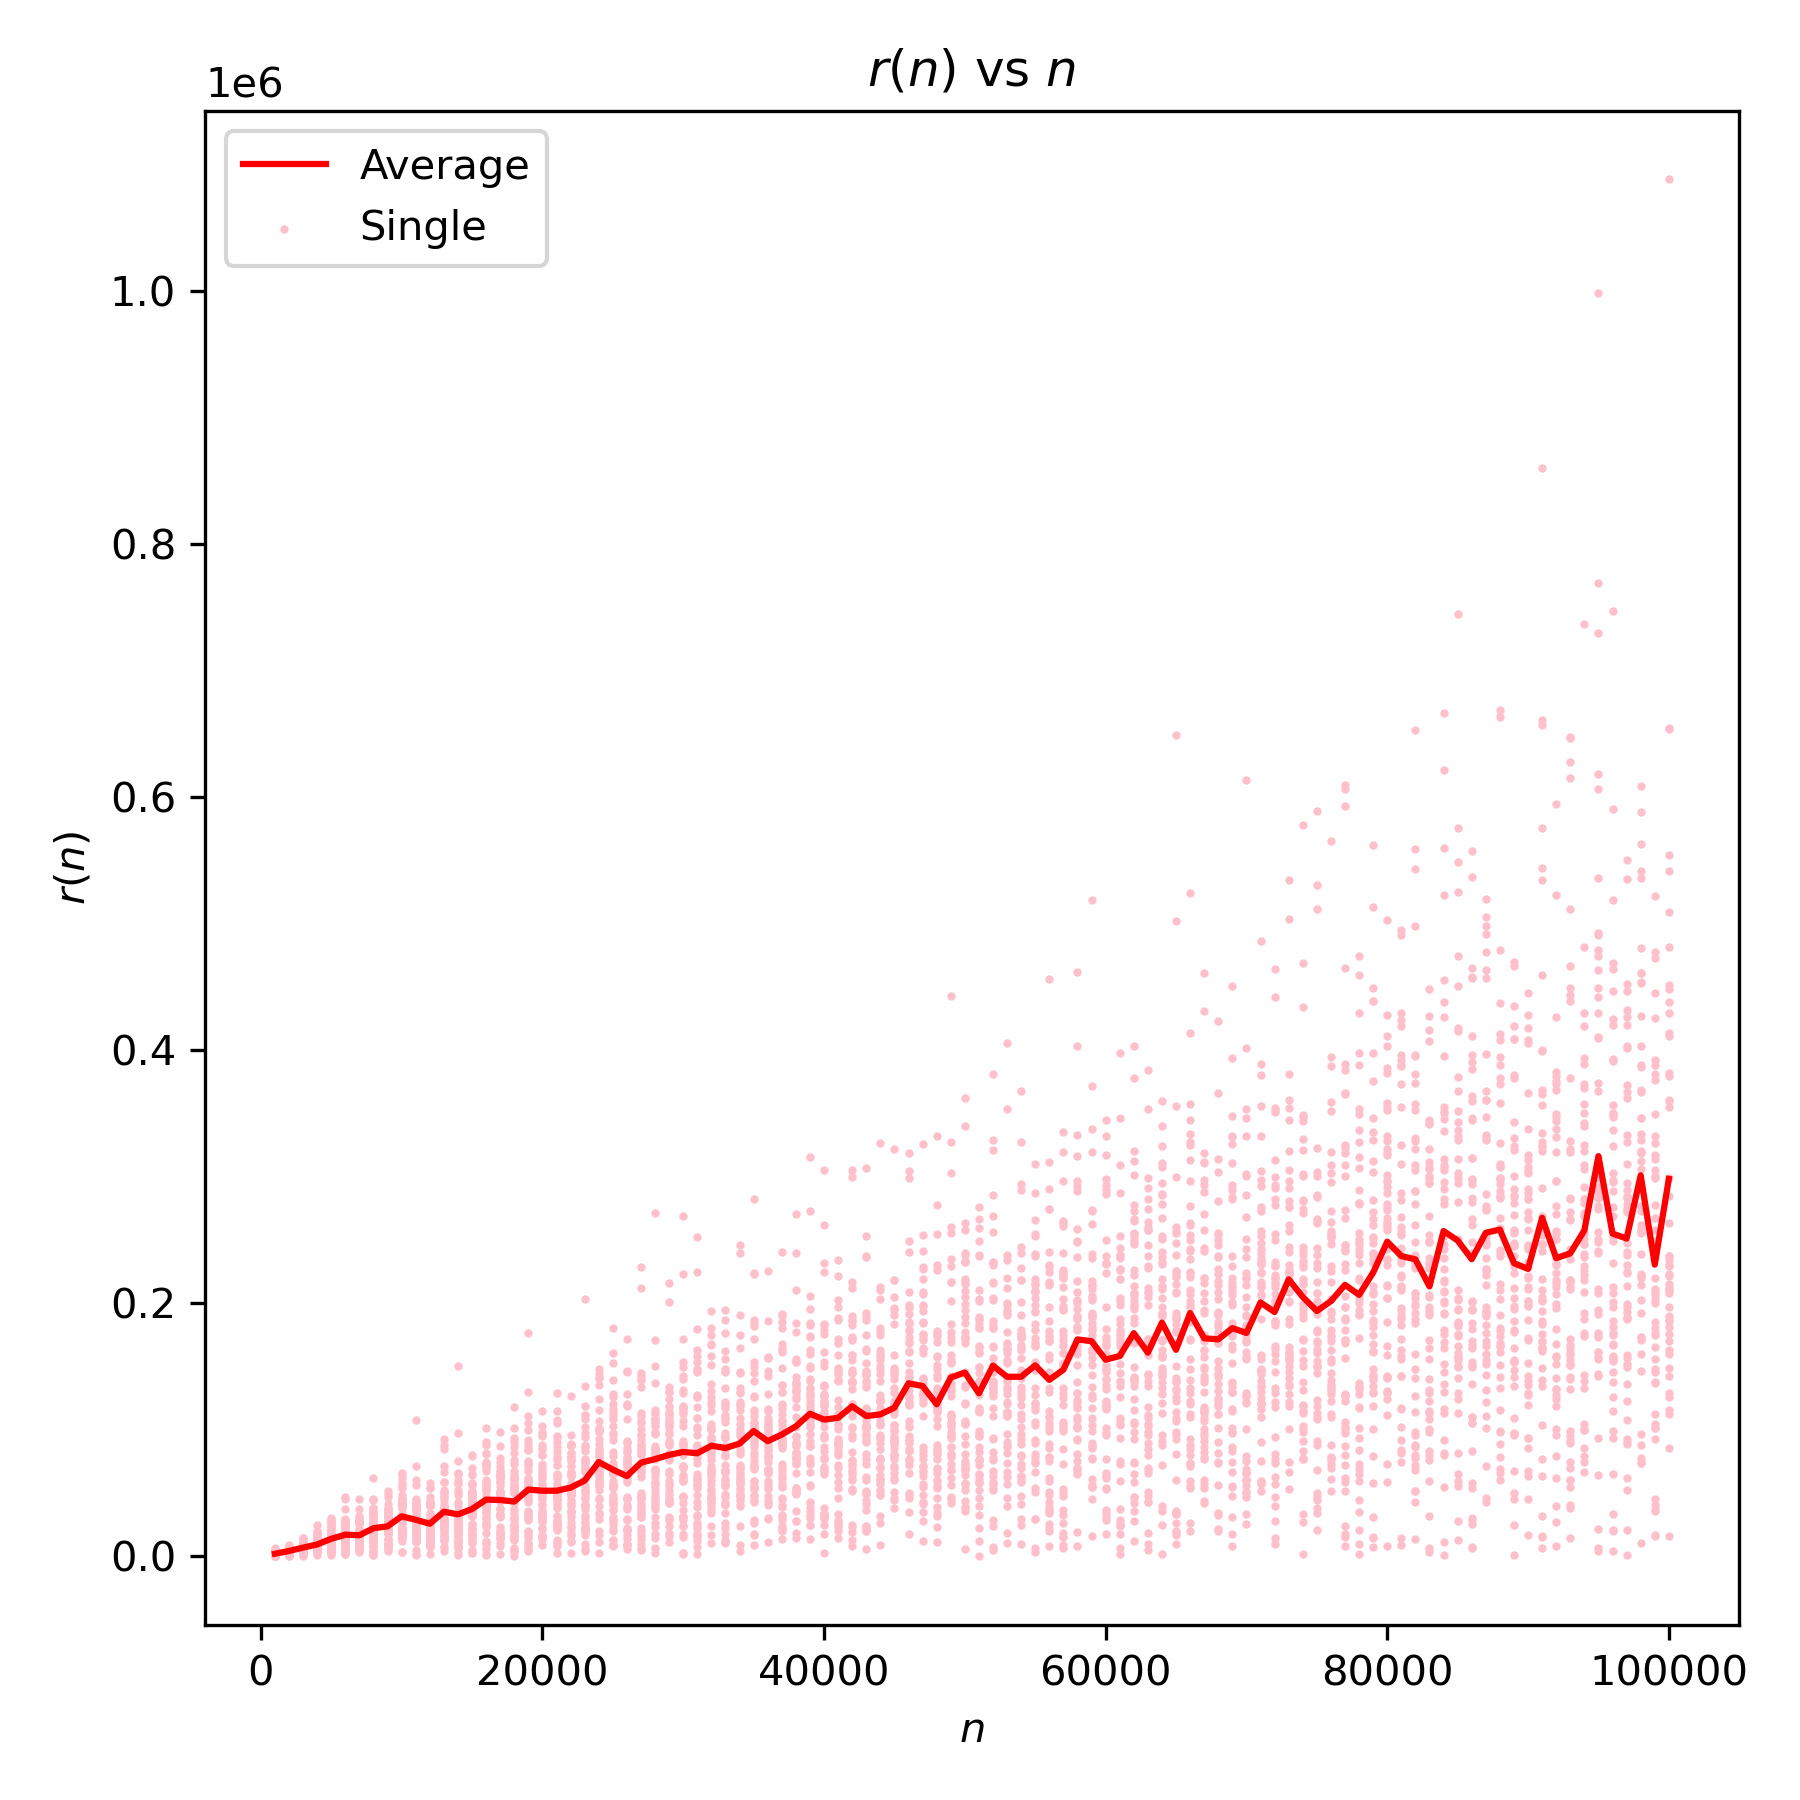
\includegraphics[width=\linewidth]{r_factor_vs_n.png}
        \caption{$R(n)=D(n)-C(n)$}
    \end{minipage}
        \begin{minipage}{0.24\textwidth}
        \centering
        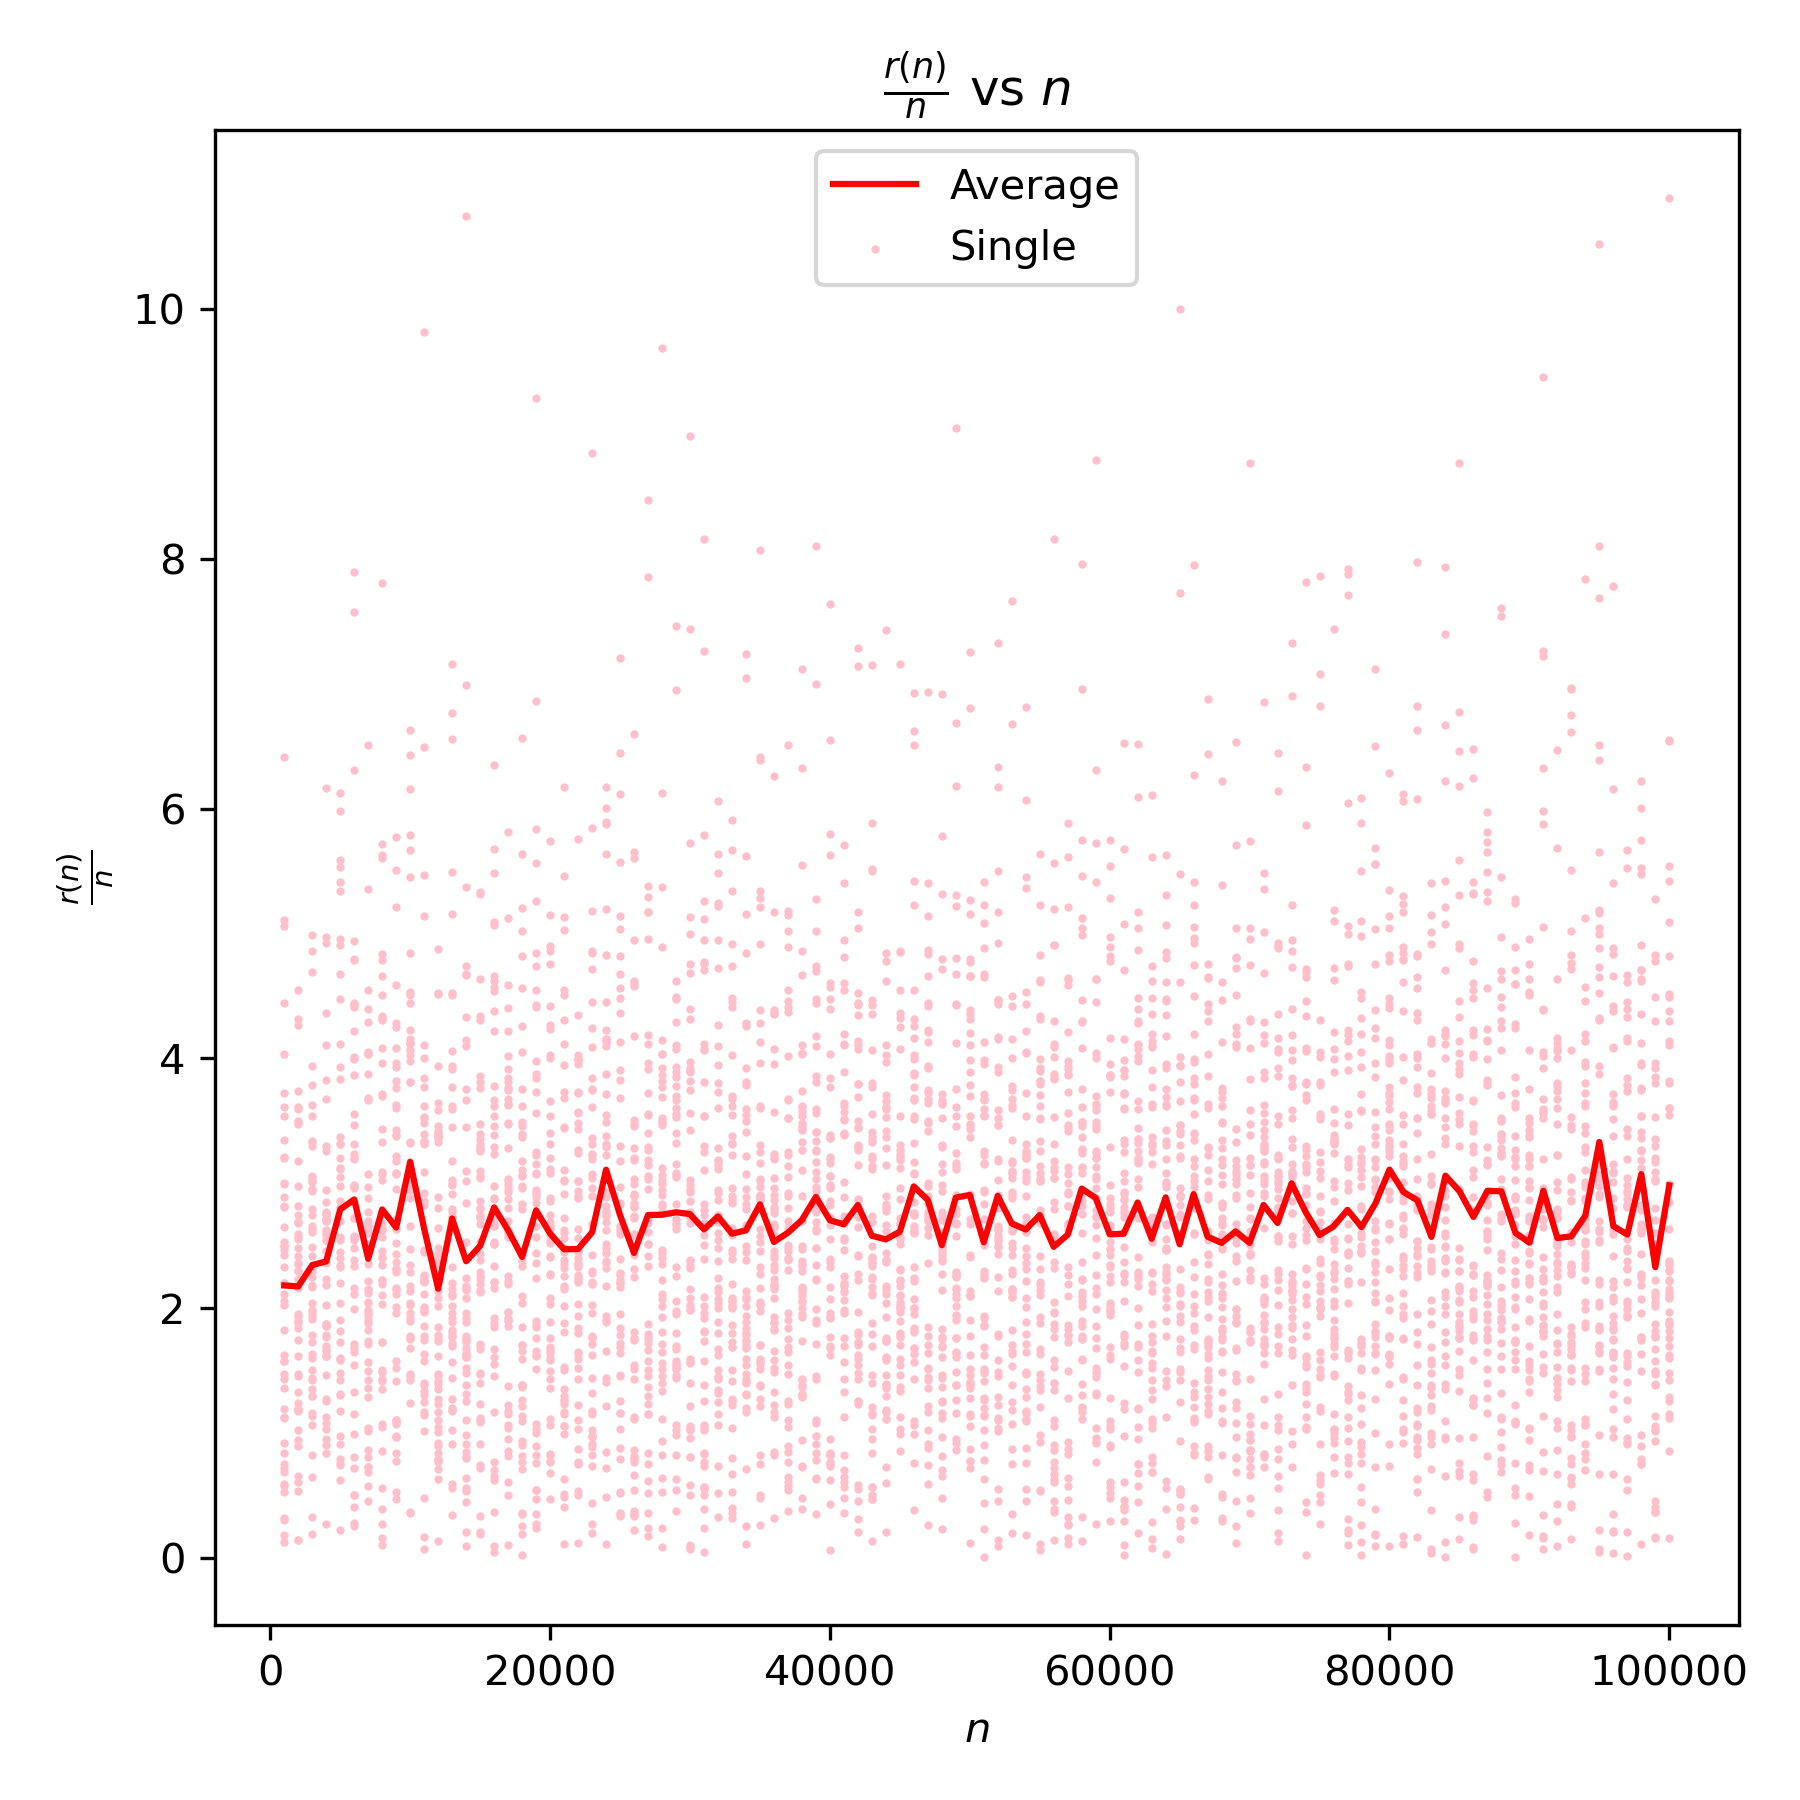
\includegraphics[width=\linewidth]{r_factor_over_n_vs_n.png}
        \caption{$\frac{r(n)}{n}$}
    \end{minipage}
        \begin{minipage}{0.24\textwidth}
        \centering
        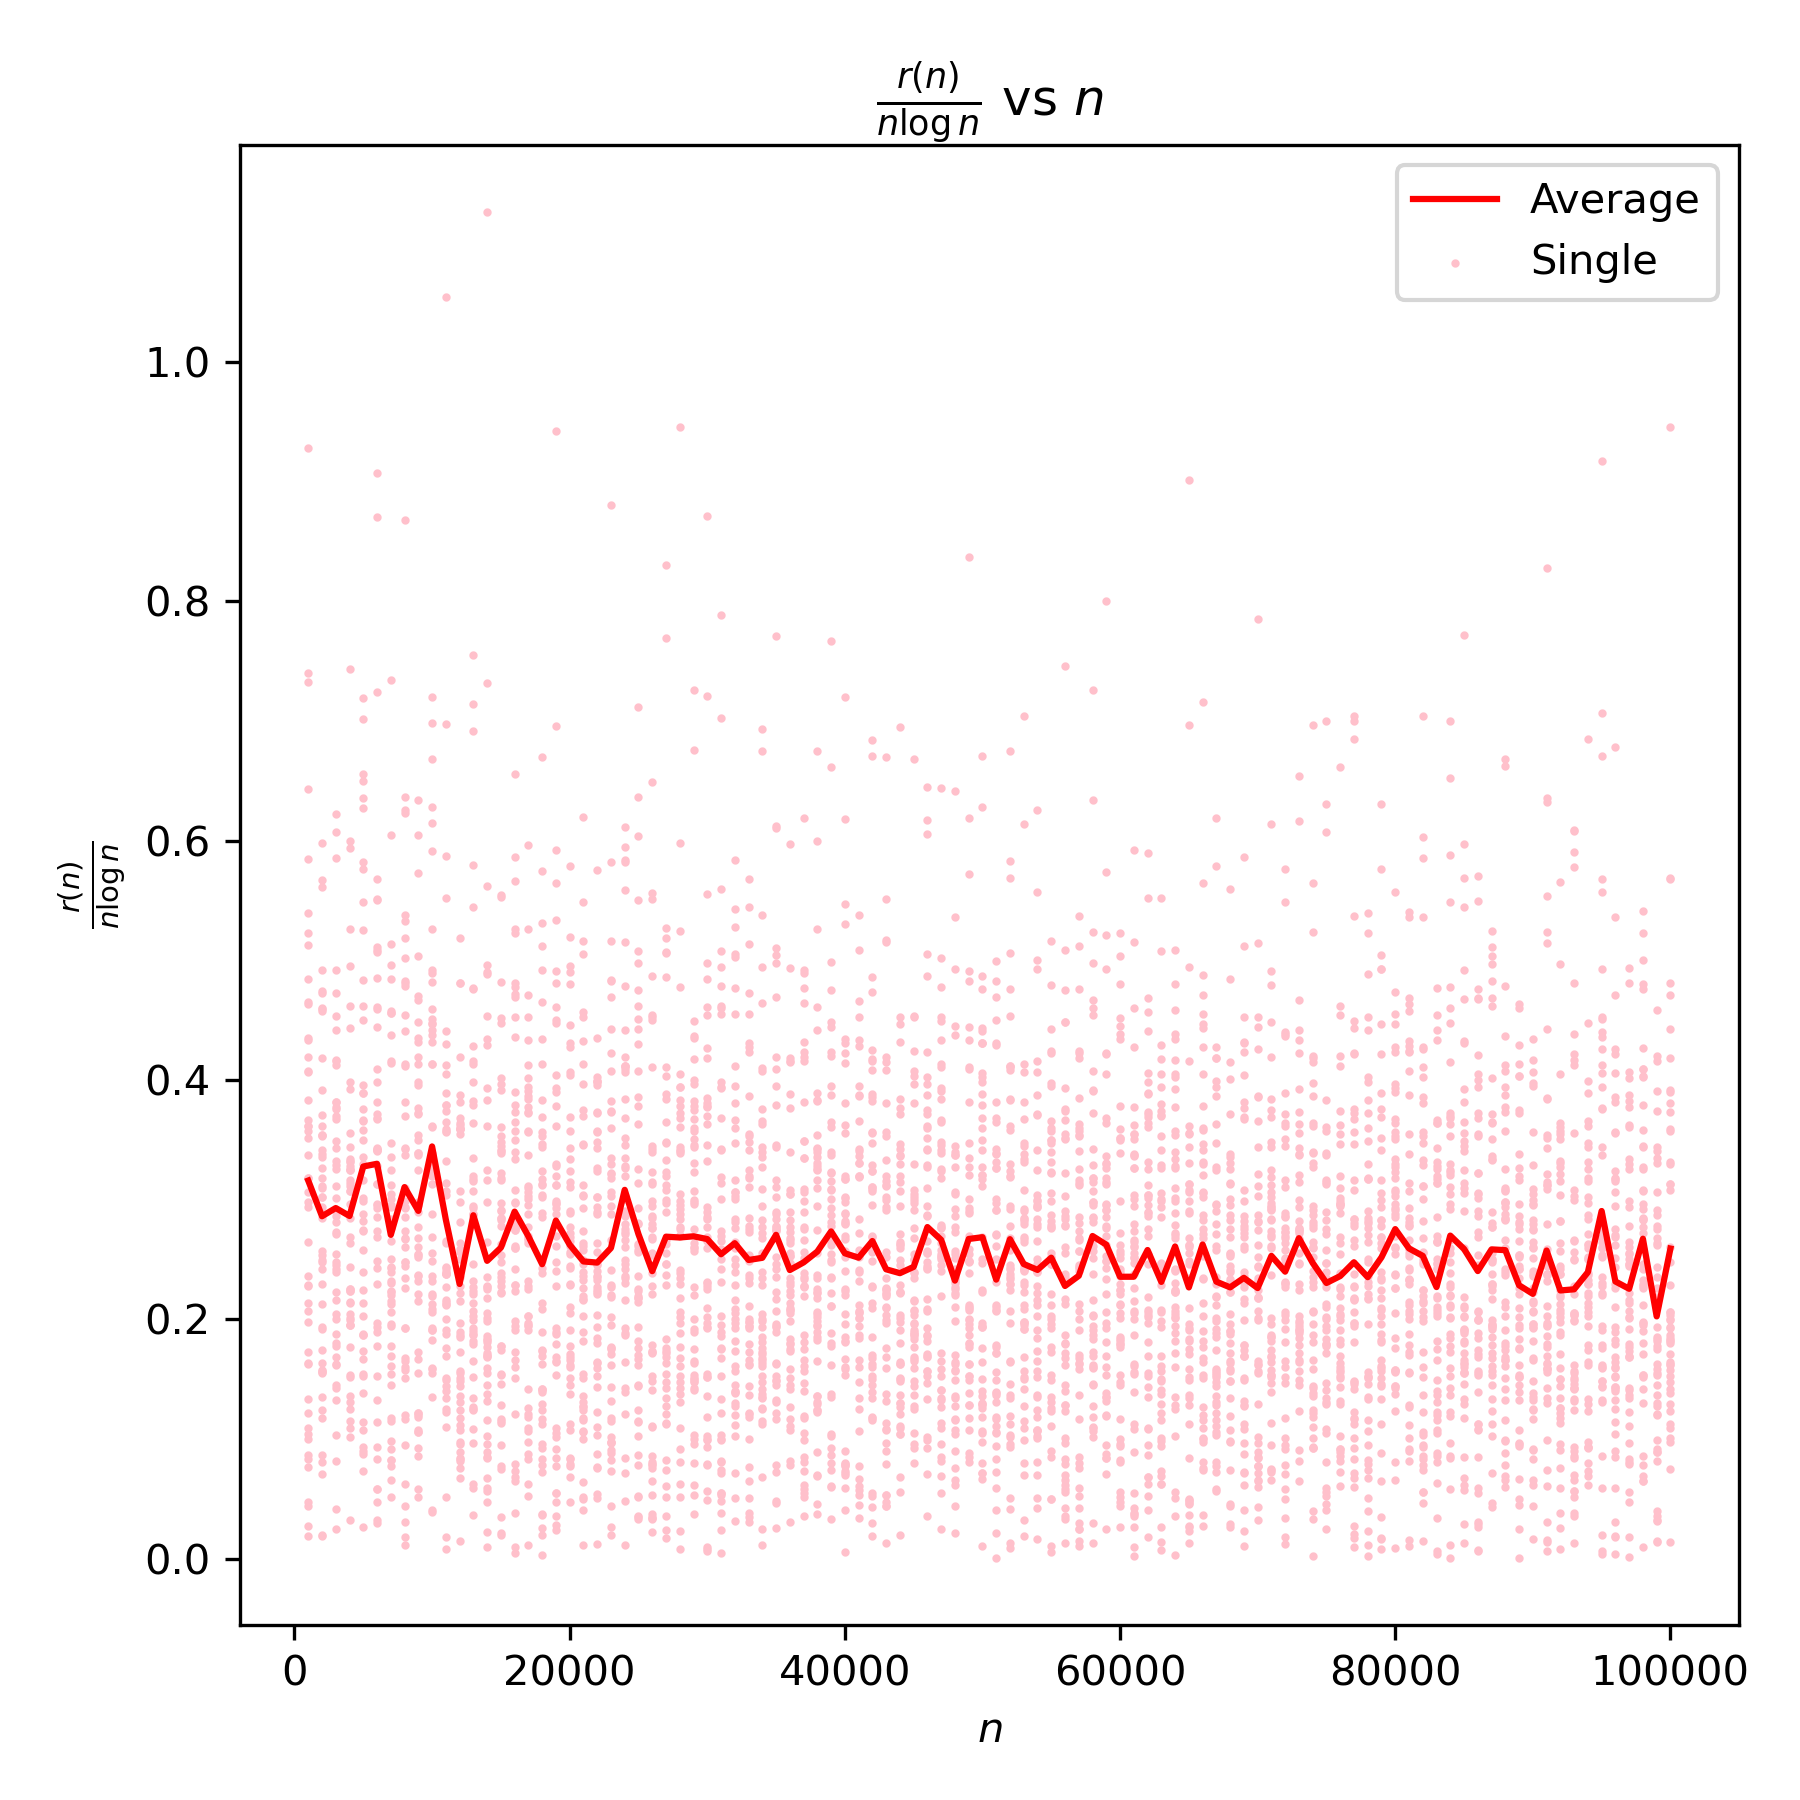
\includegraphics[width=\linewidth]{r_factor_over_n_log_n_vs_n.png}
        \caption{$\frac{r(n)}{n \log(n)}$}
    \end{minipage}
    \begin{minipage}{0.24\textwidth}
        \centering
        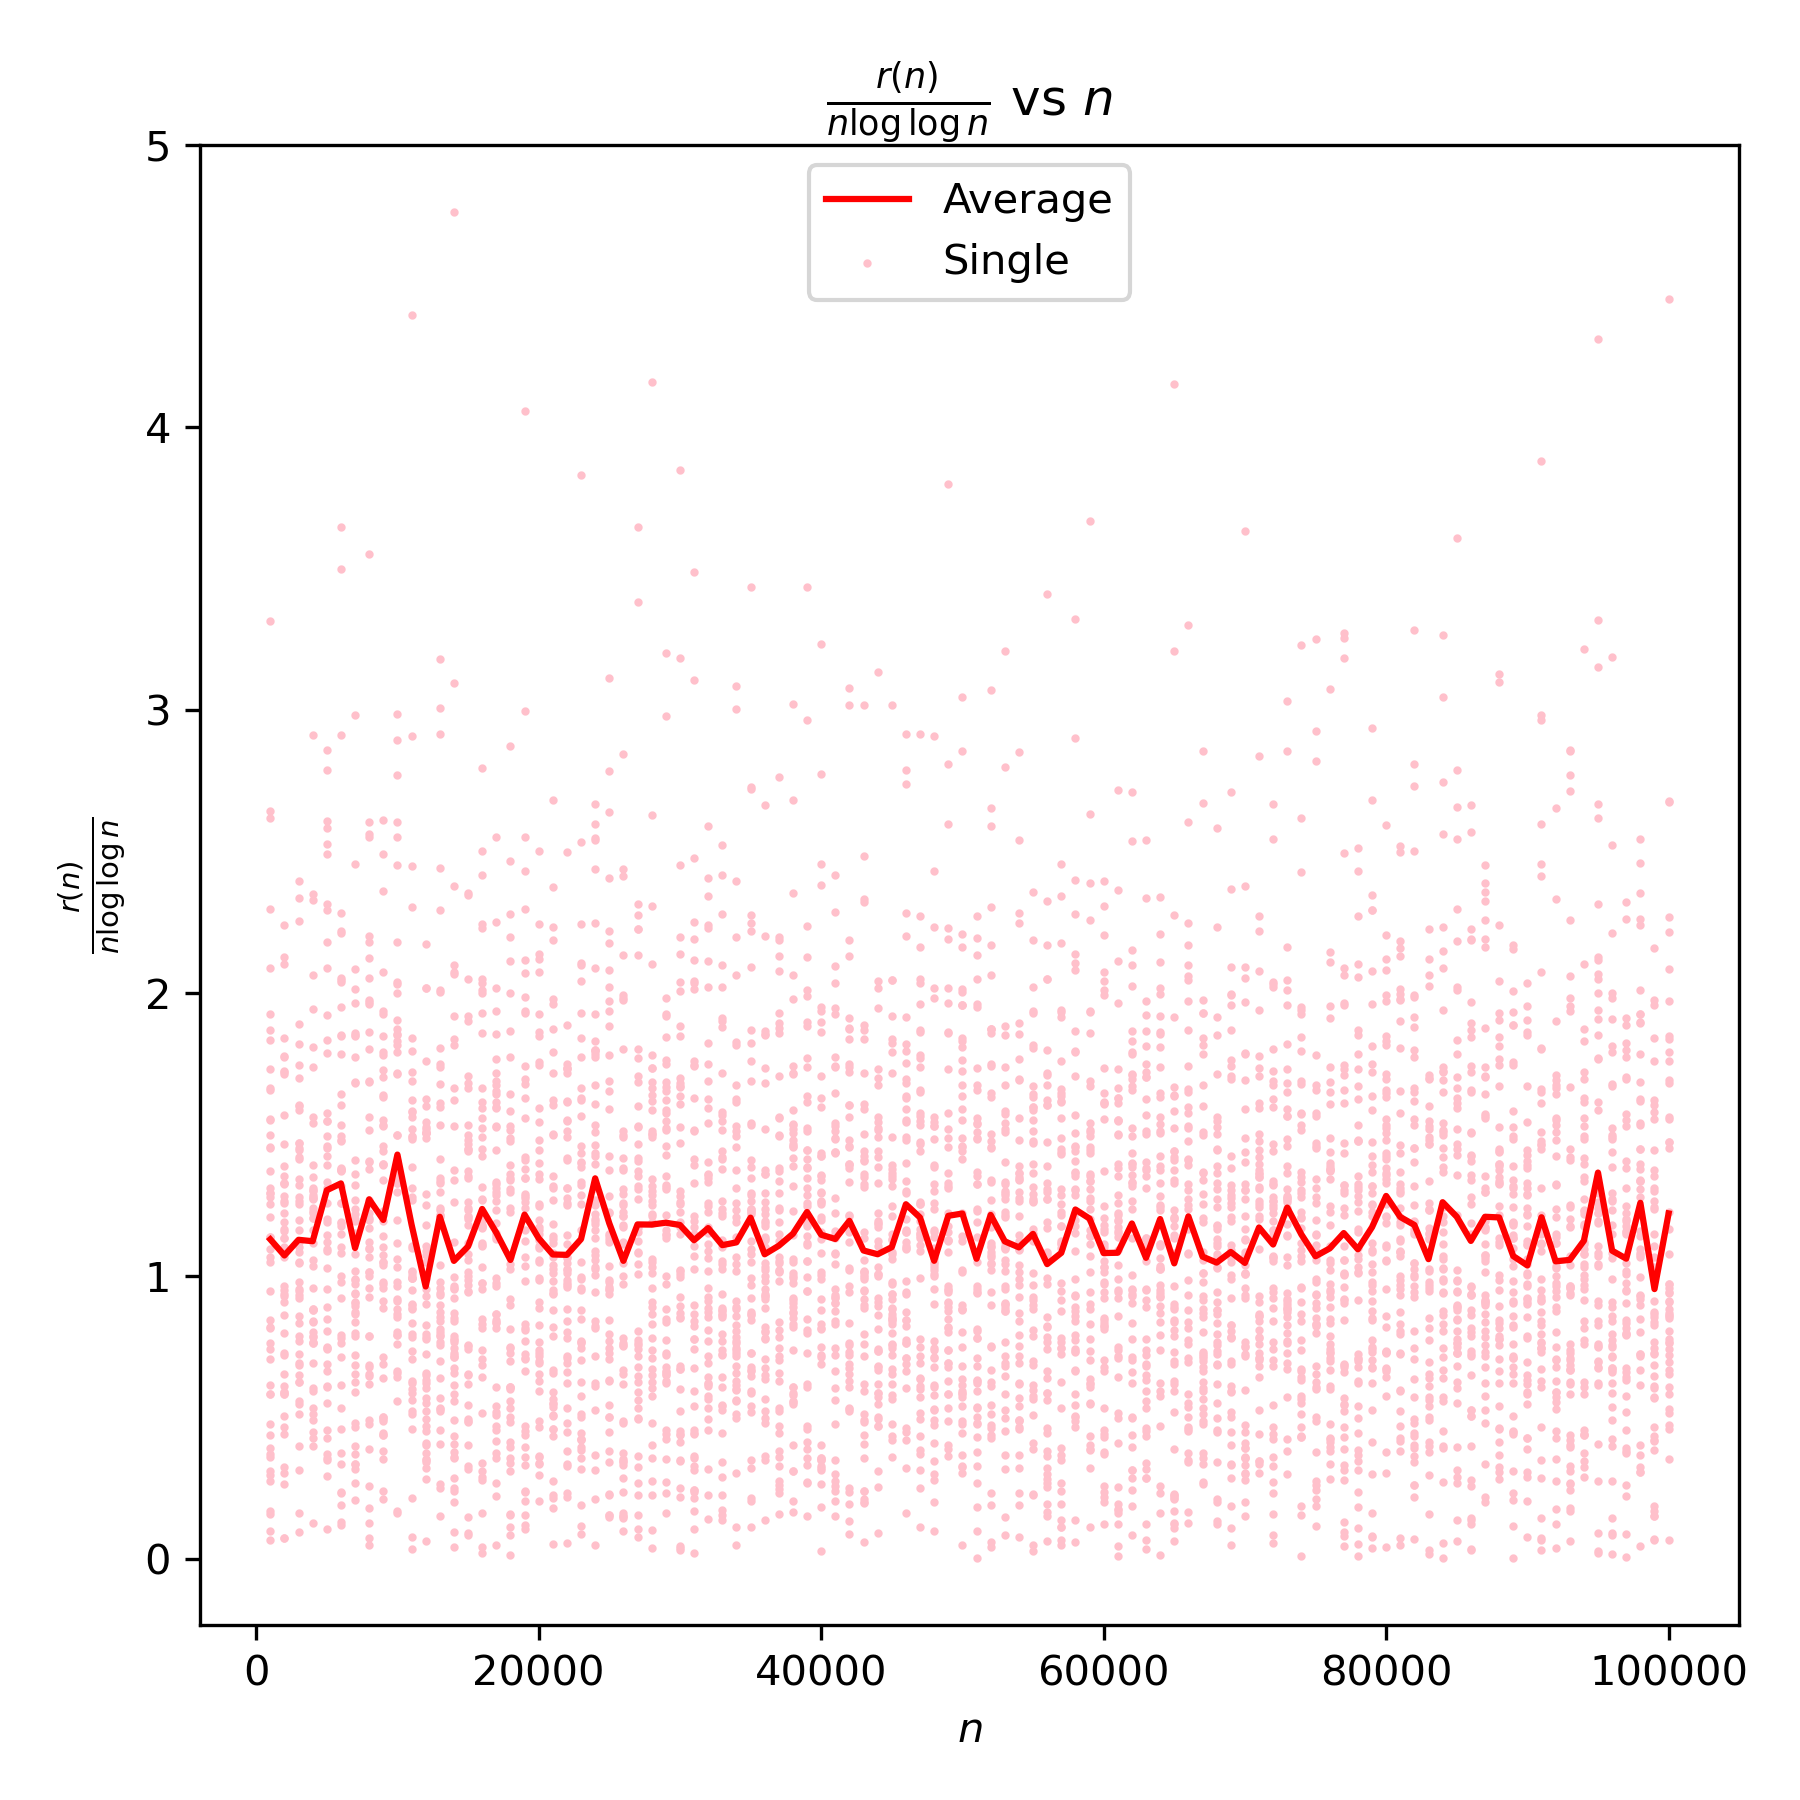
\includegraphics[width=\linewidth]{r_factor_over_n_log_log_n_vs_n.png}
        \caption{$\frac{r(n)}{n \log(\log(n))}$}
    \end{minipage}
\end{figure}

\section{Zadanie 2}

\subsection{Rezultaty}

\subsubsection{Omówienie rezultatów}

W zadaniu pierwszym zostały zaprezentowane wykresy obrazujące wyniki poszczególnych symulacji oraz wartości średnich mierzonych parametrów. Wykonane dla nich symulacje oraz uśrednione wyniki dla każdego $n$ pozwalają na wysnucie hipotez dotyczących asymptotyki wartości średnich badanych wielkości.

\subsubsection{Koncentracja wyników wokół wartości średniej}

Wraz ze wzrostem $n$ widzimy wyraźne ekspansje przedziałów w jakich znajdują się wyniki poszczególnych wartości mierzonych na wykresach liniowych. Wskazać tu można na wartości parametów $B, C, D, R$. Jest to zdarzenie oczekiwane, związane ściśle z ilością możliwych wartości które może przyjąć zmienna losowa pojedyńczego rzutu kuli. Im większe $n$, tym bardziej rozrzuconych wyników należy się spodziewać. Dopiero przy wyznaczonych średnich ze wszystkich $k=50$ przypadków możemy zaobserwować istotne tendencje.

W przypadku zdarzenia $U$ nie widzimy jednak dużego rozstrzału wyników z poszczególnych prób.

\subsubsection{Hipotezy odnośnie asymptotyki badanych wielkości}

Znając dwa poniższe fakty:

\begin{fact}{Big O Limit}
    Niech $f,g \in\mathbb{N}\rightarrow\mathbb{R}^{+}$. Zachodzi:
    \[f(n)=O(g) \iff \limsup_{n\rightarrow\infty} \frac{f(n)}{g(n)} < \infty\]
\end{fact}

\begin{fact}{Big Theta Limit}
    Niech $f,g \in\mathbb{N}\rightarrow\mathbb{R}^{+}$. Zachodzi:
    \[f(n)=\Theta(g) \iff \left(\limsup_{n\rightarrow\infty} \frac{f(n)}{g(n)} < \infty \right) \land \left(\limsup_{n\rightarrow\infty} \frac{f(n)}{g(n)} > 0 \right)\]
\end{fact}
Możemy wysnuć hipotezy na temat zależności poszczególych mierzonych wartości od parametru $n$:

\begin{enumerate}
    \item Moment pierwszej kolizji. Skoro wartości na wykresie z rysunku 3-go $\frac{b(n)}{\sqrt{n}}$ utrzymują się w niewielkim przedziale, to hipoteza: $b(n) = \Theta(\sqrt{n})$
    \item Liczba pustych urn. Ze względu na wykres z rysunku 5-go możemy napisać hipoteze: $u(n) = \Theta(n)$
    \item Minimalna liczba rzutów, po której w każdej z urn jest co najmniej jedna kula. Z rysunku 9-go możemy hipotetycznie określić asymptotykę na $c(n) = \Theta(n\ln n)$
    \item Minimalna liczba rzutów, po której w każdej z urn są co najmniej dwie kule. Z rysunku 13-go możemy hipotetycznie ocenić asymptotykę $d(n)=\Theta(n\ln n)$
    \item Różnica dwóch powyższych. Rysunki 15 oraz 17 są bardzo podobne, wobec tego w tej próbce danych możemy wysnuć dwie hipotezy $r(n)=d(n)-c(n)=\Theta(n)$ lub $r(n)=\Theta(n\log\log n)$. Wykresy są zbyt zbliżone do siebie, abym mógł z większą pewnością wybrać jeden z nich.
\end{enumerate}

\subsubsection{Intuicje stojące za nazwami \textit{Birthday paradox} oraz \textit{Coupon collector's problem}}

\textit{Birthday Paradox} - Opisuje zaskakująco wysokie prawdopodobieństwo, że w relatywnie niewielkiej grupie osób znajdą się dwie osoby, które mają urodziny w tym samym dniu. Matematyka wskazuje, że w grupie zaledwie 23 osób prawdopodobieństwo, że dwie z nich będą miały urodziny tego samego dnia, wynosi około 50\%. Jest to wynik nieoczekiwany i sprzeczny z początkową intuicją.

\textit{Coupon collector's problem} - Opisuje ile pojedyńczych kuponów musi losowo zebrać kolekcjoner aby móc cieszyć się pełną kolekcja. Aby mieć co najmniej jeden egzemplarz każdego typu, zbieracz musi podjąć znacznie więcej prób, niż wynosi liczba uniklanych kuponów.

\subsubsection{Znaczenie \textit{Birthday paradox} w kontekście funkcji hashujących}

\textit{Birthday paradox} znacząco zmniejsza ilość wymaganych prób do znalezienia kolizji (dwóch różnych argumentów dla których funkcja zwraca ten sam wynik) w funkcjach hashujących, wykorzystywanych w większości systemów informatycznych. Jak wiadomo mają one postać skończonych ciągów bitów, wobec tego dla funkcji zwracająych krótkie ciągi możliwe jest relatywnie szybkie znalezienie dwóch różnych ciągów wejściowych generujących taki sam hash. Zadaniem kryptograficznych funkcji hashujących jest zatem wytworzenie wysokiej odporności na takie przypadki, które potencjalnie mogą prowadzić na przykład do przyznania nieautoryzowanych dostępów (hash hasła znajduje się w bazie danych pewnego serwisu). Rozwiązaniem jest stworzenie funkcji hashującej zwracającej większą liczbę bitów np $SHA256$, bądź $SHA512$.

\subsection{Wnioski}

Symulacja odpowiada na zadane pytania oraz prezentuje wystarczający zestaw danych na wysnucie hipotez dotyczących asymptotyki wartości średnich badanych wielkości z dokładnością do $\Theta$. Symulacja prezentuje również przyczynę sprzężonego z nią problemu - istotnego znaczenia \textit{Birthday Paradox} w łamaniu funkcji hashujących.

\end{document}